\label{ch:results}
To validate the proposed cooperative multi-drone architecture, a comprehensive testing campaign was conducted. The evaluation follows this approach: first planners and controllers are validated in a simulated environment, then the human-in-the-loop haptic interactions are analyzed, and finally the complete cooperative mission is shown. A preliminary assessment of the physical real-world setup concludes the chapter.

\section{Software-in-the-Loop Setup}
The simulated validation was performed using the Gazebo physics engine, fully integrated with the PX4 Autopilot Software-in-the-Loop (SITL) environment and ROS 2 Humble. The multi-vehicle setup relies on the Micro-XRCE-DDS bridge to independently handle the uORB messaging for two virtual standard \texttt{x500} quadrotor frames. 
\\To replicate the computational constraints of the real onboard companion computer, the NMPC solver was configured with a strict execution constraint of $100$ Hz (sampling time $T_s = 10$ ms) over a prediction horizon of $N=15$ steps. The state and control weighting matrices ($\mathbf{Q}$ and $\mathbf{R}$) were tuned empirically to prioritize visual constraints (e.g., locking the relative height and radial distance) while heavily penalizing aggressive torque variations, ensuring a smooth video feed. 
\begin{table}[htbp]
\centering
\caption{Parameters and weight matrices in NMPC. Notice: $\Delta_{max}$, used for weights normalization, is intended as maximum acceptable displacement with respect correspondent reference}
\label{tab:nmpc_parameters}
\small
\begin{tabular}{llcccc}
\toprule
 \textbf{Symbol} & \textbf{Range $\Delta_{\max}$} & \textbf{Priority $w$} & \textbf{Value (Scalar/Diagonal)} \\
\midrule
\multicolumn{4}{l}{} \\
$T_s$            & ---                                   & ---                   & \SI{10}{\milli\second} (\SI{100}{\hertz}) \\
$N$              & ---                                   & ---                   & $15$ \\
$T_p = N T_s$    & ---                                   & ---                   & \SI{0.5}{\second} \\
\midrule
\multicolumn{4}{l}{\textit{State cost terms ($Q$)}} \\
$p_{x}, p_{y}$   & \SI{0.20}{\meter}                     & $10.0$                & $250.0$ \\
$p_{z}$          & \SI{0.15}{\meter}                     & $10.0$                & $444.4$ \\
$\psi$           & $\pi/4\ \si{\radian}$ (\ang{45})      & $10.0$                & $16.21$ \\
$v_x, v_y, v_z$  & \SI{0.20}{\meter\per\second}          & $2.0$                 & $50.0$ \\
$\omega_x, \omega_y$ & \SI{0.15}{\radian\per\second}     & $0.20$                & $8.89$ \\
$\omega_z$       & \SI{0.40}{\radian\per\second}         & $0.20$                & $1.25$ \\
$a_x, a_y, a_z$  & \SI{0.20}{\meter\per\second\squared}  & $0.33$                & $8.33$ \\
$j_x, j_y, j_z$  & \SI{4.0}{\meter\per\second\cubed}     & $0.10$                & $6.25 \times 10^{-3}$ \\
$s_x, s_y, s_z$  & \SI{20.0}{\meter\per\second\tothe{4}} & $0.10$                & $2.50 \times 10^{-4}$ \\
\midrule
\multicolumn{4}{l}{\textit{Input cost terms ($R$)}} \\
$F_z$            & \SI{0.50}{\newton}                    & $0.10$                & $0.40$ \\
$\tau_x, \tau_y$ & \SI{0.20}{\newton\meter}              & $0.10$                & $2.50$ \\
$\tau_z$         & \SI{0.50}{\newton\meter}              & $0.10$                & $0.40$ \\
\bottomrule
\end{tabular}
\end{table}


\section{NMPC Hovering and Tracking Validation}
Before introducing the autonomous switching references or human commands, a baseline validation of the Observer Drone's NMPC was performed. The objective of this isolated test is to demonstrate the stability of the optimal solver, the safety of the PID-to-NMPC switch, and the real-time computational feasibility.
\\During this test, the drone performs an autonomous vertical takeoff using the native PX4 position controller. Upon reaching the predefined hovering altitude, the safe-switch logic brings the drone into offboard thrust and torque mode. The only conceptual difference is that after the switch the observer drone keeps the other drone centered in image plane; this is a design choice. Another one could have been ignoring the yaw, that is, compensating for it and shifting it a way not to turn.
\begin{figure}[h!]
\centering
\begin{subfigure}[b]{0.51\textwidth}
    
\includegraphics[width=\linewidth]{Immagini/Capitolo6/Simulations/Hovering/phases_legend.pdf}
\end{subfigure}
\begin{subfigure}[b]{0.49\textwidth}
    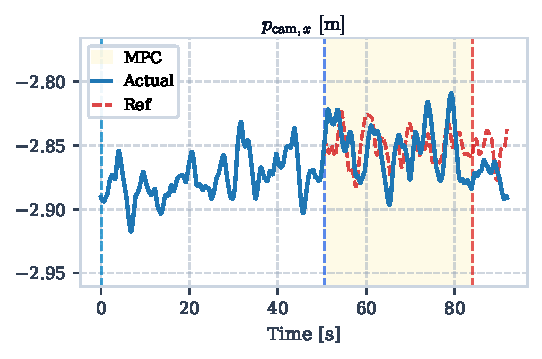
\includegraphics[width=\linewidth]{Immagini/Capitolo6/Simulations/Hovering/POS_cam_x.pdf}
    \label{fig:placeholder}
\end{subfigure}
\begin{subfigure}[b]{0.49\textwidth}
    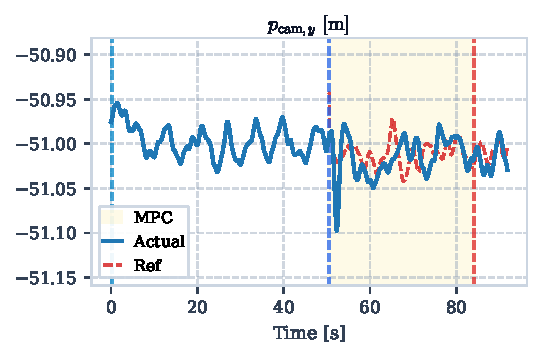
\includegraphics[width=\linewidth]{Immagini/Capitolo6/Simulations/Hovering/POS_cam_y.pdf}
    \label{fig:placeholder}
\end{subfigure}
\begin{subfigure}[b]{0.49\textwidth}
    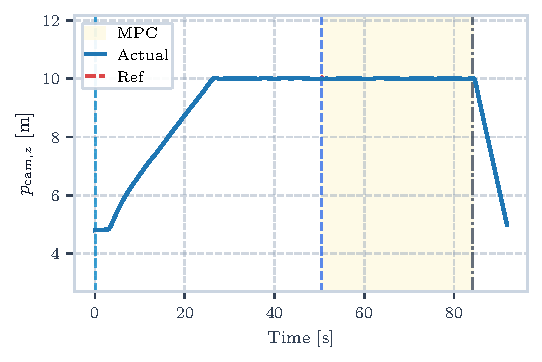
\includegraphics[width=\linewidth]{Immagini/Capitolo6/Simulations/Hovering/POS_cam_z.pdf}
    \label{fig:placeholder}
\end{subfigure}
\begin{subfigure}[b]{0.49\textwidth}
    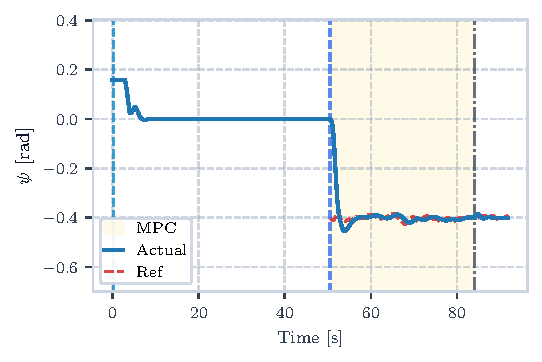
\includegraphics[width=\linewidth]{Immagini/Capitolo6/Simulations/Hovering/YAW_yaw_actual_vs_desired.pdf}
    \label{fig:placeholder}
\end{subfigure}
\caption{Cartesian coordinates of Observer Drone camera in ENU frame}
\label{fig:hovering_pos}
\end{figure}
\\As shown in Figure \ref{fig:hovering_pos}, the NMPC successfully maintains the hovering flight dynamics. Mostly important, the transition between the two controllers is without any transient instability or loss of altitude. 
The yaw smoothly reaches a zero-error steady state, while 3D position of the drone is kept around hovering position, with performances comparable to the standard PID-hovering.
\begin{figure}[h!]
\centering
\begin{subfigure}[b]{0.51\textwidth}
    
\includegraphics[width=\linewidth]{Immagini/Capitolo6/Simulations/Hovering/phases_legend.pdf}
\end{subfigure}
\begin{subfigure}[b]{0.49\textwidth}
    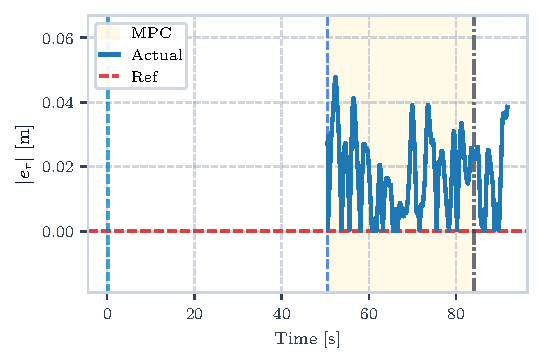
\includegraphics[width=\linewidth]{Immagini/Capitolo6/Simulations/Hovering/CYL_POV_ERR_distance_error_r_cyl_err.pdf}
    \label{fig:placeholder}
\end{subfigure}
\begin{subfigure}[b]{0.49\textwidth}
    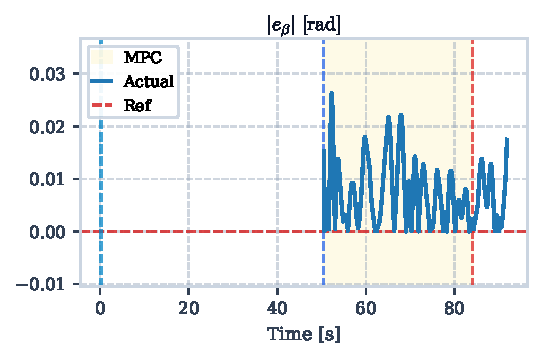
\includegraphics[width=\linewidth]{Immagini/Capitolo6/Simulations/Hovering/CYL_POV_ERR_azimuth_error_beta_err.pdf}
    \label{fig:placeholder}
\end{subfigure}
\begin{subfigure}[b]{0.49\textwidth}
    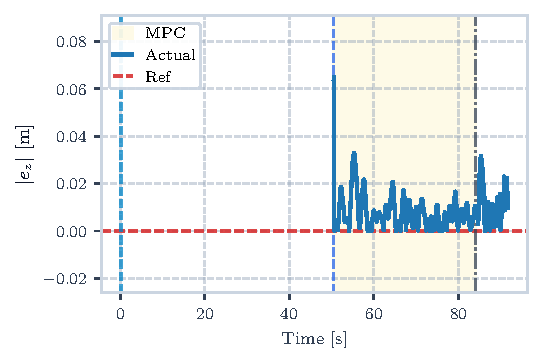
\includegraphics[width=\linewidth]{Immagini/Capitolo6/Simulations/Hovering/CYL_POV_ERR_elevation_error_z_err.pdf}
    \label{fig:placeholder}
\end{subfigure}
\begin{subfigure}[b]{0.49\textwidth}
    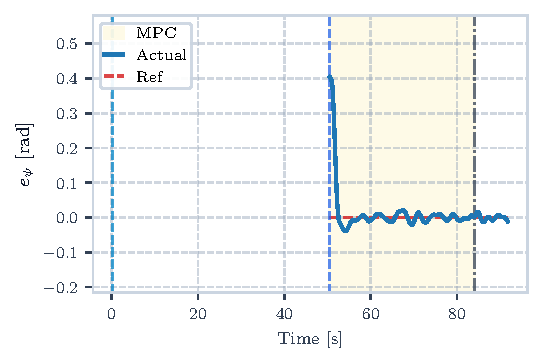
\includegraphics[width=\linewidth]{Immagini/Capitolo6/Simulations/Hovering/YAW_yaw_error.pdf}
    \label{fig:placeholder}
\end{subfigure}
\caption{Error norms - Cylindrical position and yaw orientation}
\label{fig:hovering_err}
\end{figure}
\\The observer drone pose shown in \ref{fig:hovering_pos} is computed based on visual references, that are cylindrical ones. For this reason figure \ref{fig:hovering_err} shows cylindrical errors, minimized in the NMPC cost function.
\begin{figure}[h!]
\centering
\begin{subfigure}[b]{0.51\textwidth}
    
\includegraphics[width=\linewidth]{Immagini/Capitolo6/Simulations/Hovering/phases_legend.pdf}
\end{subfigure}
\begin{subfigure}[b]{0.49\textwidth}
    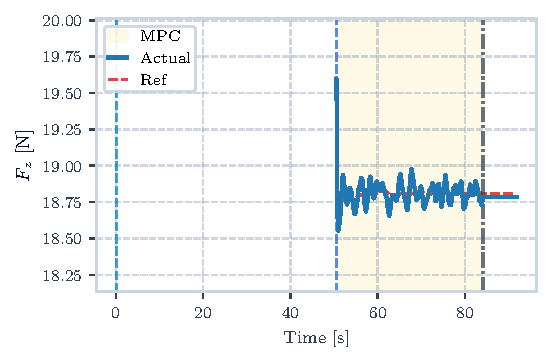
\includegraphics[width=\linewidth]{Immagini/Capitolo6/Simulations/Hovering/CONTROL_WRENCH_force_z.pdf}
    \label{fig:placeholder}
\end{subfigure}
\begin{subfigure}[b]{0.49\textwidth}
    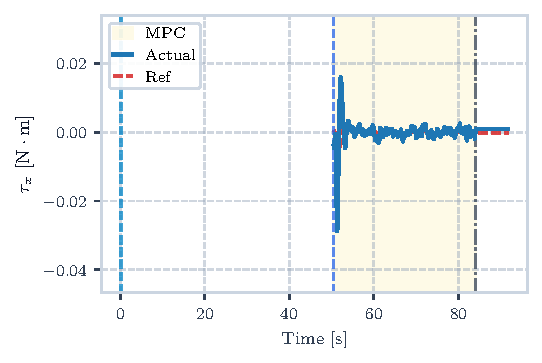
\includegraphics[width=\linewidth]{Immagini/Capitolo6/Simulations/Hovering/CONTROL_WRENCH_torque_x.pdf}
    \label{fig:placeholder}
\end{subfigure}
\begin{subfigure}[b]{0.49\textwidth}
    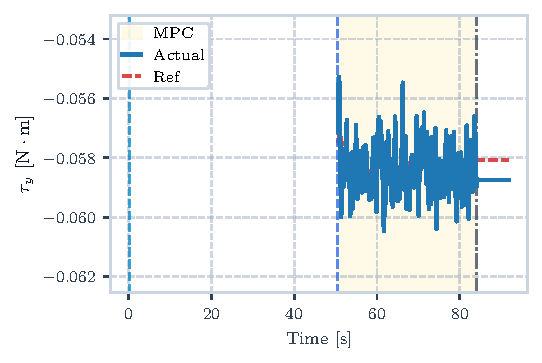
\includegraphics[width=\linewidth]{Immagini/Capitolo6/Simulations/Hovering/CONTROL_WRENCH_torque_y.pdf}
    \label{fig:placeholder}
\end{subfigure}
\begin{subfigure}[b]{0.49\textwidth}
    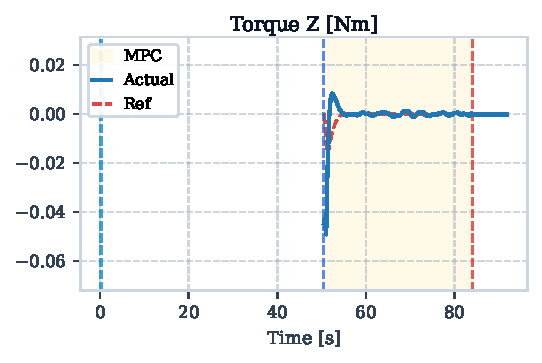
\includegraphics[width=\linewidth]{Immagini/Capitolo6/Simulations/Hovering/CONTROL_WRENCH_torque_z.pdf}
    \label{fig:placeholder}
\end{subfigure}
\caption{Hovering - Control wrench}
\label{fig:control_switch}
\end{figure}
Figure \ref{fig:control_switch} illustrates the body thrust and torques during the switch phase. Also thanks to the safety check over Euclidean distance between the PID-computed outputs and the NMPC-predicted outputs, so that it falls below the safety threshold $\epsilon$, the control signals remain perfectly continuous. This result is very important, since one of the main objective of the MPC controller was to consider actuation constraints inside the problem and thrust and torques are the real outputs of this controller. \\It is worth to notice that control torque $\tau_y$ oscillates around a value different from 0. This is due to model mismatches, precisely to a camera umodeled displacement with respect to CoM. This doesn't represent a problem, anyway, since both this and other disturbances can be handled by the MBE (\ref{fig:MBE}) that, regardless, brings tracking errors to 0.
\begin{figure}[h!]
\centering
\begin{subfigure}[b]{0.71\textwidth}
    
\includegraphics[width=\linewidth]{Immagini/Capitolo6/Simulations/Hovering/phases_legend.pdf}
\end{subfigure}
\begin{subfigure}[b]{0.32\textwidth}
    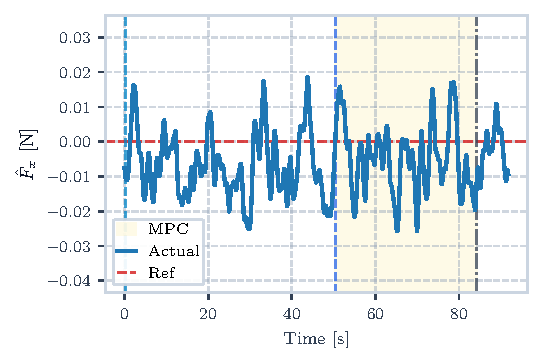
\includegraphics[width=\linewidth]{Immagini/Capitolo6/Simulations/Hovering/MBE_force_x.pdf}
    \label{fig:placeholder}
\end{subfigure}
\begin{subfigure}[b]{0.32\textwidth}
    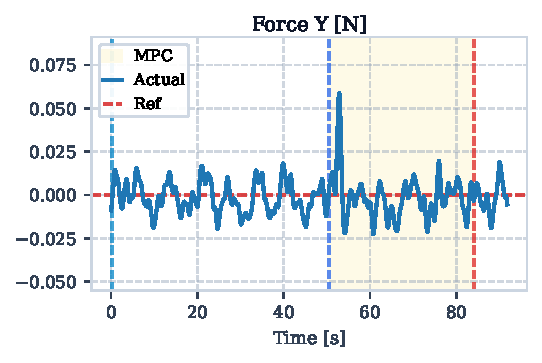
\includegraphics[width=\linewidth]{Immagini/Capitolo6/Simulations/Hovering/MBE_force_y.pdf}
    \label{fig:placeholder}
\end{subfigure}
\begin{subfigure}[b]{0.32\textwidth}
    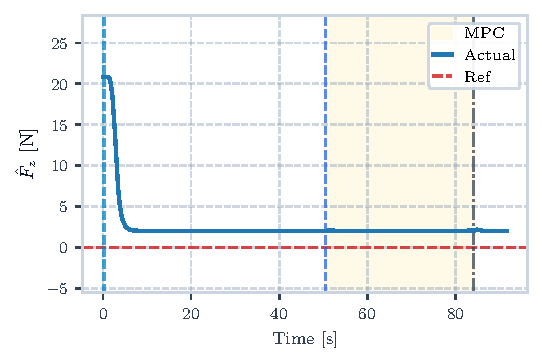
\includegraphics[width=\linewidth]{Immagini/Capitolo6/Simulations/Hovering/MBE_force_z.pdf}
    \label{fig:placeholder}
\end{subfigure}
\begin{subfigure}[b]{0.32\textwidth}
    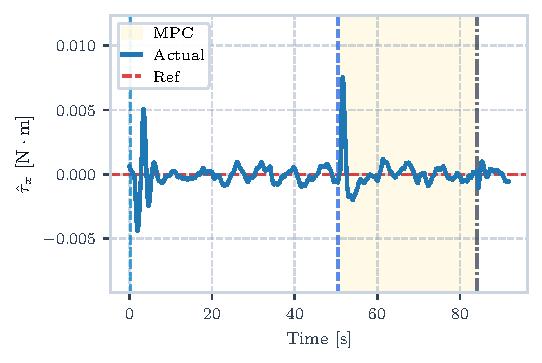
\includegraphics[width=\linewidth]{Immagini/Capitolo6/Simulations/Hovering/MBE_torque_x.pdf}
    \label{fig:placeholder}
\end{subfigure}
\begin{subfigure}[b]{0.32\textwidth}
    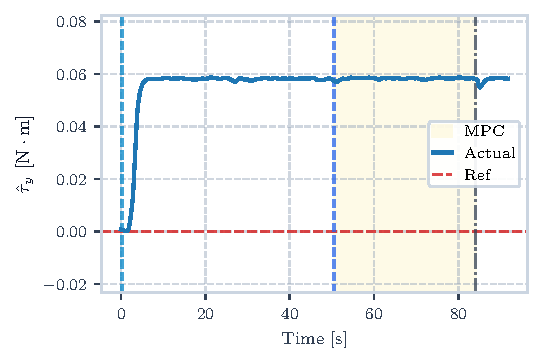
\includegraphics[width=\linewidth]{Immagini/Capitolo6/Simulations/Hovering/MBE_torque_y.pdf}
    \label{fig:placeholder}
\end{subfigure}
\begin{subfigure}[b]{0.32\textwidth}
    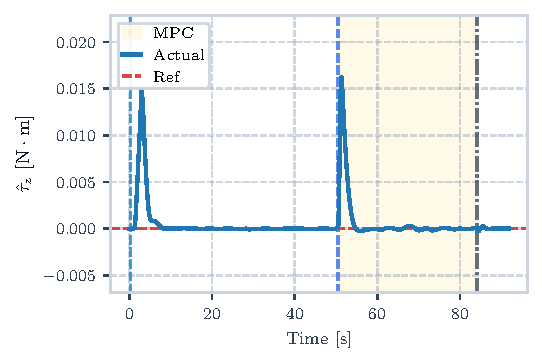
\includegraphics[width=\linewidth]{Immagini/Capitolo6/Simulations/Hovering/MBE_torque_z.pdf}
    \label{fig:placeholder}
\end{subfigure}
\caption{Hovering - Momentum Based Estimator, external estimated wrenches}
\label{fig:MBE}
\end{figure}

\subsection{Computational Efficiency}
Real-time feasibility is a strict requirement for aerial optimal control. A statistical analysis of the solver's execution time over the entire flight log confirms the extreme efficiency of the C-generated Acados code. 
\begin{figure}[h!]
\centering
\begin{subfigure}[b]{0.51\textwidth}
    
\includegraphics[width=\linewidth]{Immagini/Capitolo6/Simulations/Hovering/phases_legend.pdf}
\end{subfigure}
\begin{subfigure}[b]{0.8\textwidth}
    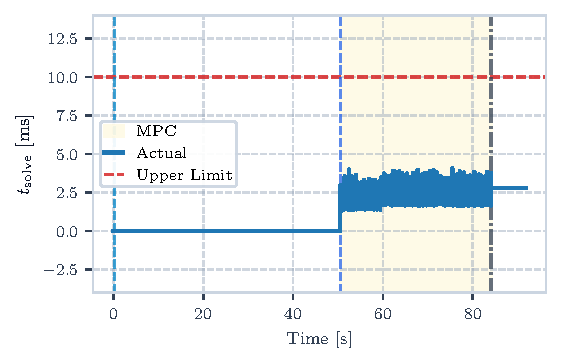
\includegraphics[width=\linewidth]{Immagini/Capitolo6/Simulations/Hovering/SOLVE_TIME_solve_time.pdf}
    \label{fig:placeholder}
\end{subfigure}
\caption{Hovering - NMPC Solving time}
\label{fig:solve_time}
\end{figure}
The NMPC cycle recorded an average execution time of $2.20$ ms, with a worst-case peak of $4.07$ ms. Since the solver must complete its routine within the $10$ ms discretization window ($T_s$), the system achieved a $0\%$ overrun rate. This is an important result for safely bringing the architecture over the onboard companion computer.

\section{Haptic Bilateral Teleoperation}
Having validated the baseline hovering stability of the NMPC, the second testing phase isolates and evaluates the human-machine interface. The objective is to demonstrate how the human operator can dynamically alter the Observer Drone's Point of View (PoV) via the Novint Falcon, and how the system safely handles conflicting inputs through force feedback.
\\During this test, the human operator uses the haptic device to command continuous variations of the cylindrical references: radial distance ($\rho_{ref}$), relative angular azimuth ($\beta_{ref}$), and relative height ($z_{ref}$).
\begin{figure}[h!]
\centering
\begin{subfigure}[b]{0.51\textwidth}
    
\includegraphics[width=\linewidth]{Immagini/Capitolo6/Simulations/Haptic/phases_legend.pdf}
\end{subfigure}
\begin{subfigure}[b]{0.49\textwidth}
    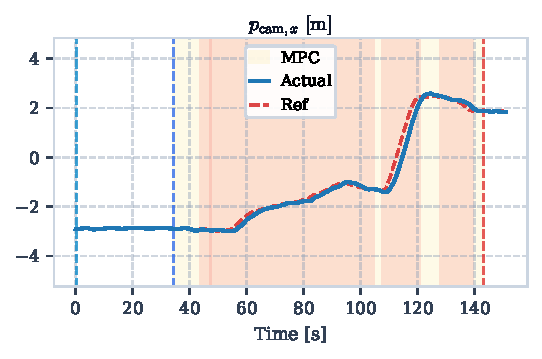
\includegraphics[width=\linewidth]{Immagini/Capitolo6/Simulations/Haptic/POS_cam_x.pdf}
    \label{fig:placeholder}
\end{subfigure}
\begin{subfigure}[b]{0.49\textwidth}
    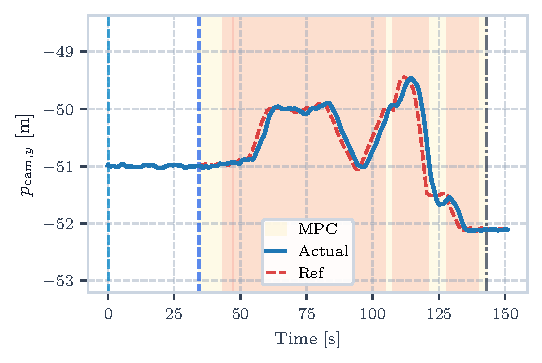
\includegraphics[width=\linewidth]{Immagini/Capitolo6/Simulations/Haptic/POS_cam_y.pdf}
    \label{fig:placeholder}
\end{subfigure}
\begin{subfigure}[b]{0.49\textwidth}
    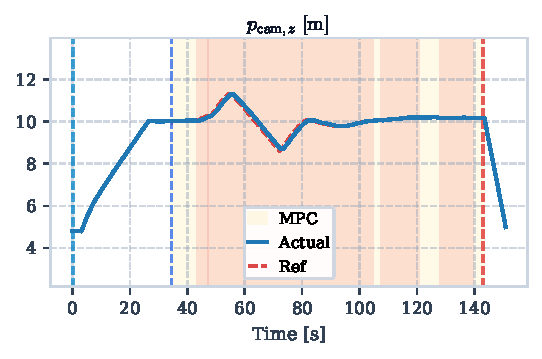
\includegraphics[width=\linewidth]{Immagini/Capitolo6/Simulations/Haptic/POS_cam_z.pdf}
    \label{fig:placeholder}
\end{subfigure}
\begin{subfigure}[b]{0.49\textwidth}
    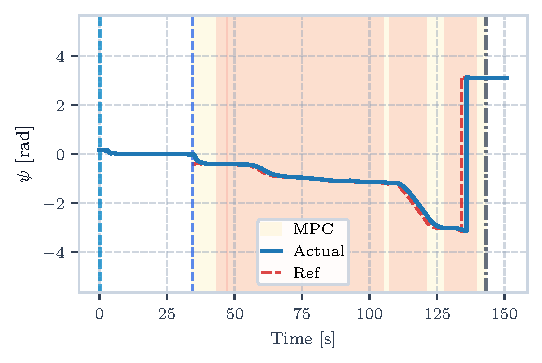
\includegraphics[width=\linewidth]{Immagini/Capitolo6/Simulations/Haptic/YAW_yaw.pdf}
    \label{fig:placeholder}
\end{subfigure}
\caption{Cartesian coordinates of Observer Drone camera in ENU frame}
\label{fig:haptic_pos}
\end{figure}
Figure \ref{fig:haptic_pos} shows the UAV's response to dynamic haptic commands.
The NMPC shows to be capable of tracking time-varying setpoints, smoothly adapting the drone's spatial position consistently with operator's intent. The mean errors across all cylindrical coordinates remain within acceptable operational margins, highlighting the absence of phase lags despite the complexity of the nonlinear optimization, as it is shown by figure \ref{fig:haptic_cyl}. There's some delay, anyway, as but it is simply due to MPC gains choice: penalizing acceleration, jerk and snap makes the flight smoother but also a bit less reactive. 
\begin{figure}[h!]
\centering
\begin{subfigure}[b]{0.51\textwidth}
    
\includegraphics[width=\linewidth]{Immagini/Capitolo6/Simulations/Haptic/phases_legend.pdf}
\end{subfigure}
\begin{subfigure}[b]{0.49\textwidth}
    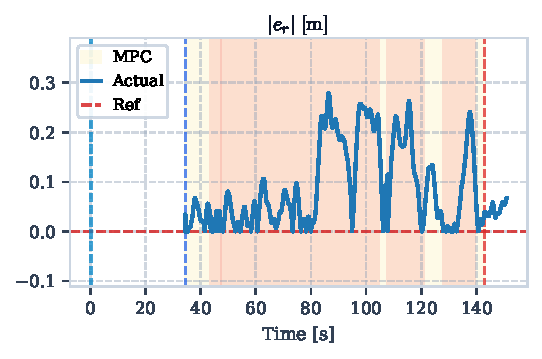
\includegraphics[width=\linewidth]{Immagini/Capitolo6/Simulations/Haptic/CYL_POV_ERR_distance_error_r_cyl_err.pdf}
    \label{fig:placeholder}
\end{subfigure}
\begin{subfigure}[b]{0.49\textwidth}
    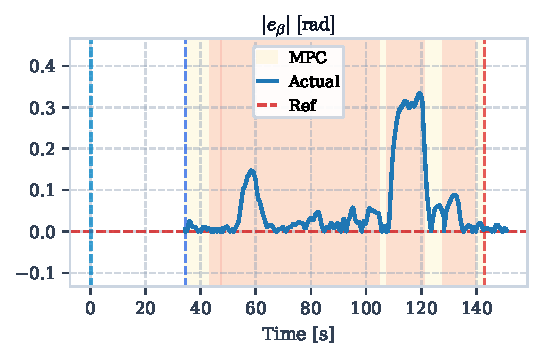
\includegraphics[width=\linewidth]{Immagini/Capitolo6/Simulations/Haptic/CYL_POV_ERR_azimuth_error_beta_err.pdf}
    \label{fig:placeholder}
\end{subfigure}
\begin{subfigure}[b]{0.49\textwidth}
    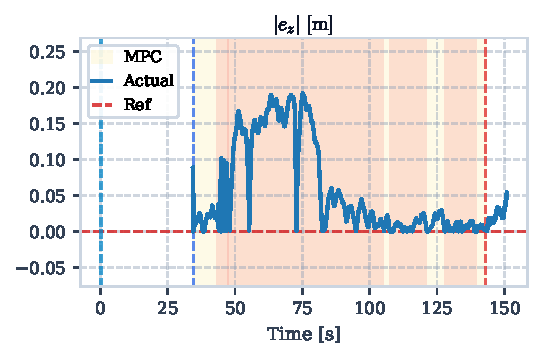
\includegraphics[width=\linewidth]{Immagini/Capitolo6/Simulations/Haptic/CYL_POV_ERR_elevation_error_z_err.pdf}
    \label{fig:placeholder}
\end{subfigure}
\begin{subfigure}[b]{0.49\textwidth}
    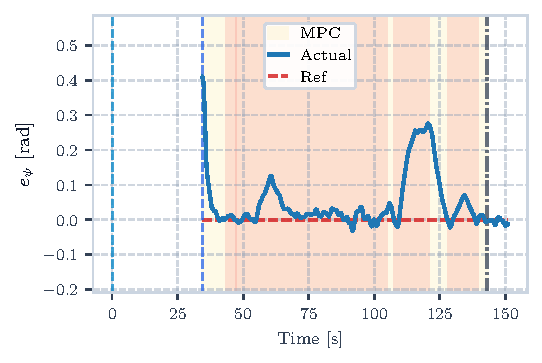
\includegraphics[width=\linewidth]{Immagini/Capitolo6/Simulations/Haptic/YAW_yaw_error.pdf}
    \label{fig:placeholder}
\end{subfigure}
\caption{Errors on cylindrical variables and yaw orientation}
\label{fig:haptic_cyl}
\end{figure}
\\However, human teleoperation commands can be unpredictable and may lead the vehicle towards unfeasible or unsafe configurations, such as bringing the Observer dangerously close to the target or causing visual loss by pushing the target outside the camera Field of View (FOV). To evaluate the Artificial Potential Field (APF) virtual fixtures, the operator deliberately commanded the drone towards the safety boundaries.

Figures~\ref{fig:APF_violations_sim} and~\ref{fig:APF_forces_sim} illustrate the resulting constraint violations and the corresponding repulsive forces rendered by the haptic device during the simulation.
\begin{figure}[h!]
\centering
\begin{subfigure}[b]{0.71\textwidth}
    
\includegraphics[width=\linewidth]{Immagini/Capitolo6/Simulations/Haptic/phases_legend.pdf}
\end{subfigure}
\begin{subfigure}[b]{0.32\textwidth}
    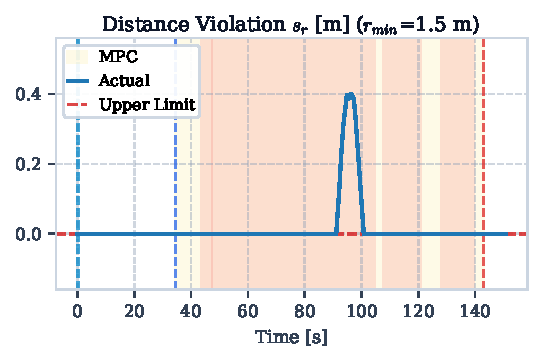
\includegraphics[width=\linewidth]{Immagini/Capitolo6/Simulations/Haptic/APF_distance_violation_s_r.pdf}
    \caption{Distance violation $s_r$}
\end{subfigure}
\begin{subfigure}[b]{0.32\textwidth}
    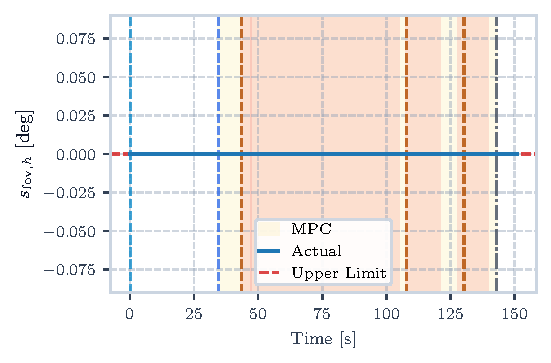
\includegraphics[width=\linewidth]{Immagini/Capitolo6/Simulations/Haptic/APF_horiz_fov_violation_s__fov_h.pdf}
    \caption{Horizontal FoV violation $s_{fov,h}$}
\end{subfigure}
\begin{subfigure}[b]{0.32\textwidth}
    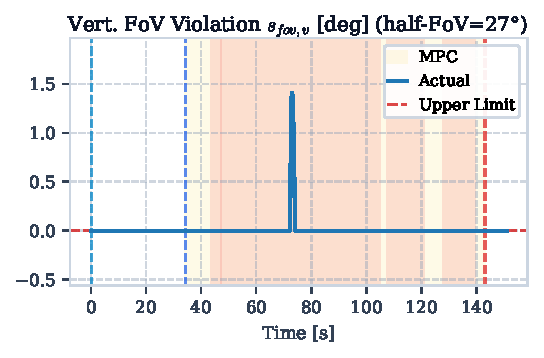
\includegraphics[width=\linewidth]{Immagini/Capitolo6/Simulations/Haptic/APF_vert_fov_violation_s__fov_v.pdf}
    \caption{Vertical FoV violation $s_{fov,v}$}
\end{subfigure}
\caption{Artificial Potential Field boundary violations during simulated haptic teleoperation}
\label{fig:APF_violations_sim}
\end{figure}

\begin{figure}[h!]
\centering
\begin{subfigure}[b]{0.71\textwidth}
    
\includegraphics[width=\linewidth]{Immagini/Capitolo6/Simulations/Haptic/phases_legend.pdf}
\end{subfigure}
\begin{subfigure}[b]{0.32\textwidth}
    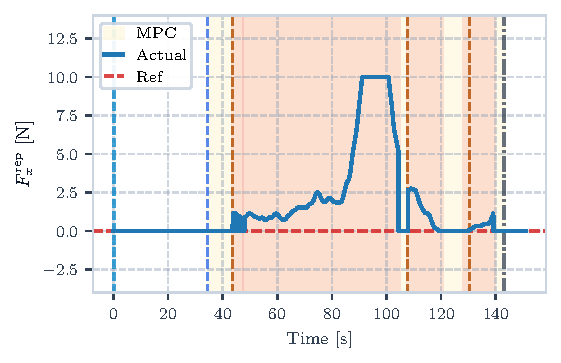
\includegraphics[width=\linewidth]{Immagini/Capitolo6/Simulations/Haptic/REPULSIVE_FORCES_repulsive_force_x.pdf}
    \caption{Radial repulsive force $F_x^{\text{rep}}$}
\end{subfigure}
\begin{subfigure}[b]{0.32\textwidth}
    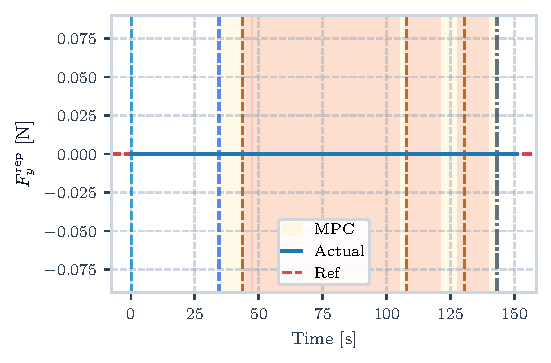
\includegraphics[width=\linewidth]{Immagini/Capitolo6/Simulations/Haptic/REPULSIVE_FORCES_repulsive_force_y.pdf}
    \caption{Azimuth repulsive force $F_y^{\text{rep}}$}
\end{subfigure}
\begin{subfigure}[b]{0.32\textwidth}
    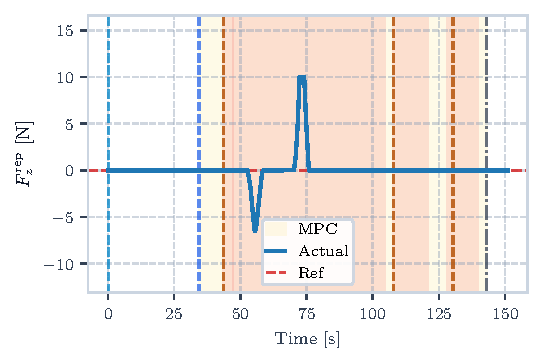
\includegraphics[width=\linewidth]{Immagini/Capitolo6/Simulations/Haptic/REPULSIVE_FORCES_repulsive_force_z.pdf}
    \caption{Elevation repulsive force $F_z^{\text{rep}}$}
\end{subfigure}
\caption{Repulsive forces rendered to the human operator via the haptic interface during simulated teleoperation}
\label{fig:APF_forces_sim}
\end{figure}

As shown in the plots, the system reliably reacts to the impending hazards:
\begin{itemize}
    \item \textbf{Radial Distance Violation ($s_r$):} Around $t \approx 91\text{ s}$, the pilot pushes the joystick forward, commanding an aggressive approach towards the Inspection UAV. As the standoff distance breaches the safety threshold $r_{\min} = 1.50\text{ m}$, the exponential repulsive force $F_x^{\text{rep}}$ rises sharply and reaches the saturation threshold of $10.0\text{ N}$ (from $t \approx 91.1\text{ s}$). The maximum encroachment reaches $s_r = 0.40\text{ m}$ at $t = 96.15\text{ s}$, meaning the inter-drone distance momentarily dropped to $r_{\text{cyl}} = 1.10\text{ m}$ (a $40\text{ cm}$ safety encroachment). The persistent tactile resistance alerts the operator to the collision hazard, prompting them to release forward pressure. As a consequence, the standoff distance smoothly recovers beyond $1.50\text{ m}$ at $t = 100.65\text{ s}$, and $s_r$ promptly returns to zero.
    \item \textbf{Vertical FoV Violation ($s_{\text{fov},v}$):} Around $t \approx 72\text{ s}$, the operator commands an upward climb, raising the Observer's altitude relative to the target. Because the camera has a fixed pitch, the target approaches the bottom boundary of the vertical Field of View ($\text{FOV}_v = 54.5^\circ$, semi-aperture $\approx 27.3^\circ$). At $t = 73.03\text{ s}$, a transient angular violation of $s_{\text{fov},v} = 1.41^\circ$ ($0.025\text{ rad}$) is recorded. Geometrically, at the current standoff distance of $r_{\text{cyl}} = 2.40\text{ m}$, the optical semi-aperture corresponds to a maximum visible semi-height of $z_{\max} = 1.24\text{ m}$, whereas the drone reached $|z_{\text{cyl}}| = 1.31\text{ m}$. This corresponds to a physical height overshoot of:
    \begin{equation}
        \Delta z = |z_{\text{cyl}}| - z_{\max} = 1.31\text{ m} - 1.24\text{ m} = 7.57\text{ cm}.
    \end{equation}
    The target thus exceeded the optical boundary by only $\approx 7.6\text{ cm}$. In response, the APF instantly delivers a downward repulsive force $F_z^{\text{rep}} = -10.0\text{ N}$ to the joystick handle. This prompt tactile cue guides the pilot to descend, recovering visual framing within just $1.8\text{ s}$ ($t = 74.09\text{ s}$).
    \item \textbf{Horizontal FoV ($s_{\text{fov},h}$):} Throughout the entire teleoperation session, the horizontal FOV violation remains strictly zero ($s_{\text{fov},h} = 0.00^\circ$, $F_y^{\text{rep}} = 0.0\text{ N}$). This confirms that the autonomous yaw tracking loop maintains the optical axis tightly aligned with the target's relative azimuth, absorbing the lateral dynamics and preventing target loss on the horizontal image plane.
\end{itemize}

\section{Complete Cooperative Mission (SITL)}
The final stage of the Software-in-the-Loop validation integrates all modules into the full dual-drone cooperative architecture. In this scenario, the Inspection Drone executes a programmed approach toward a structure, while the Observer Drone autonomously maintains the visual, guided by the NMPC and the operator's haptic supervision.
\\Moreover, the mission is planned to autonomously change visual parameters $r,\beta,z_{rel},\psi$ at each phase of the mission, according to phase visual requirements, in order to help the operator in supervising the mission itself and to teleoperate the other drone at the best of his capabilities.
\begin{figure}[h!]
    \centering
    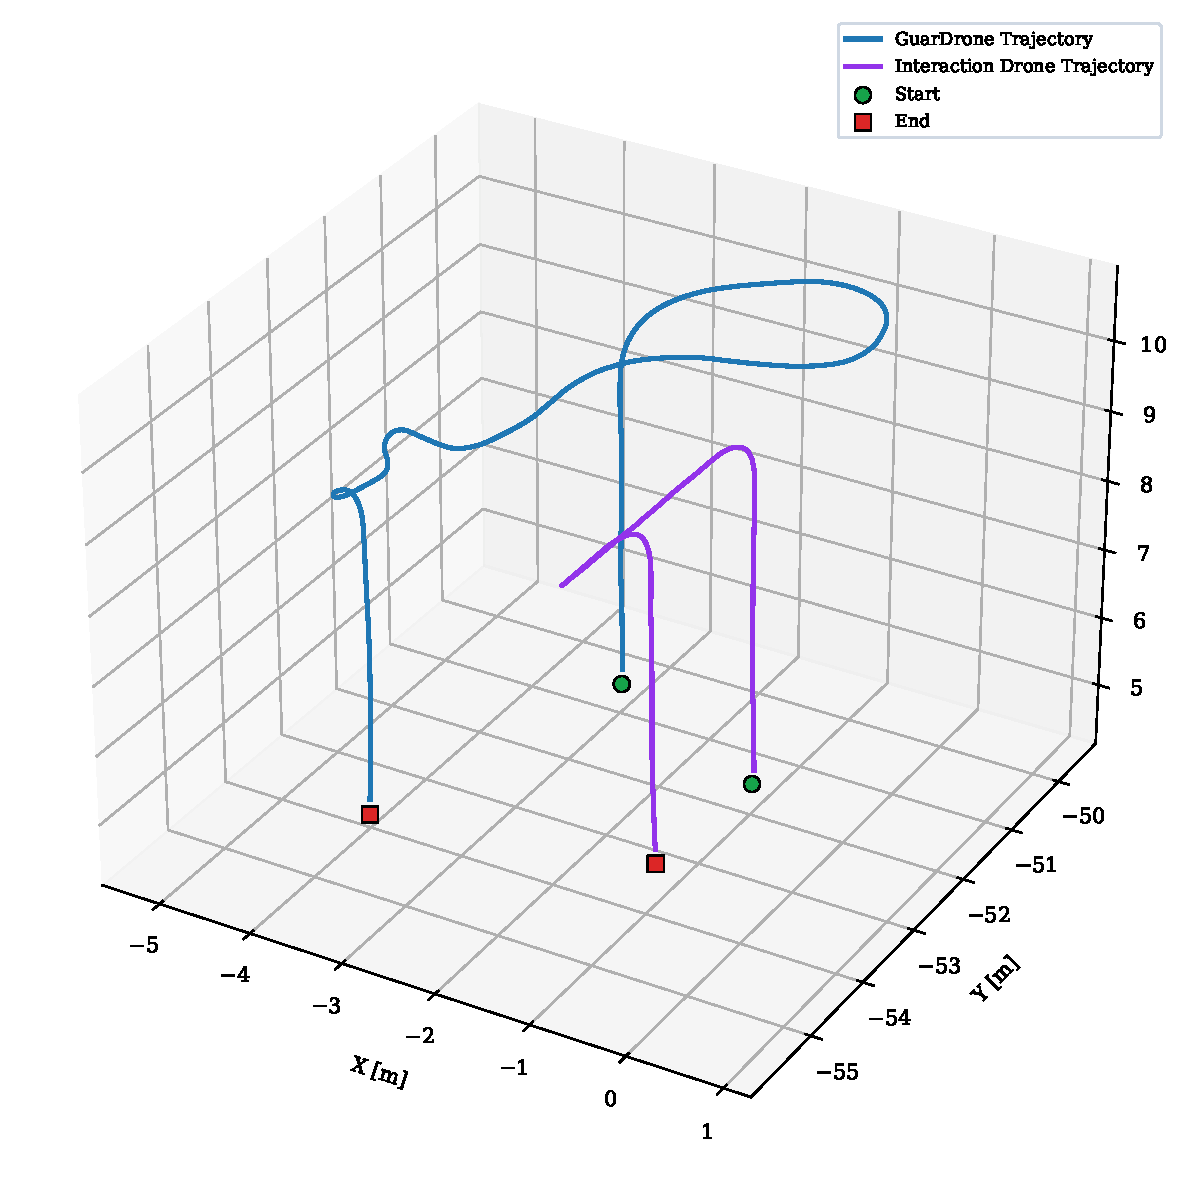
\includegraphics[width=0.5\linewidth]{Immagini/Capitolo6/Simulations/Mission/3D.pdf}
    \caption{3D trajectories of the two drones}
    \label{fig:3d_mission}
\end{figure}
The spatial evolution of the mission is captured in the 3D trajectory plot (Figure \ref{fig:3d_mission}) and in the respective Cartesian coordinates (Figures \ref{fig:mission_cam_pose} and \ref{fig:mission_int_pose}). The mission evolves through sequential operational phases governed by the FSM, depicted in Figure \ref{fig:sim_mission_phases}:

\begin{figure}[htbp]
\centering
\begin{subfigure}[b]{0.48\textwidth}
    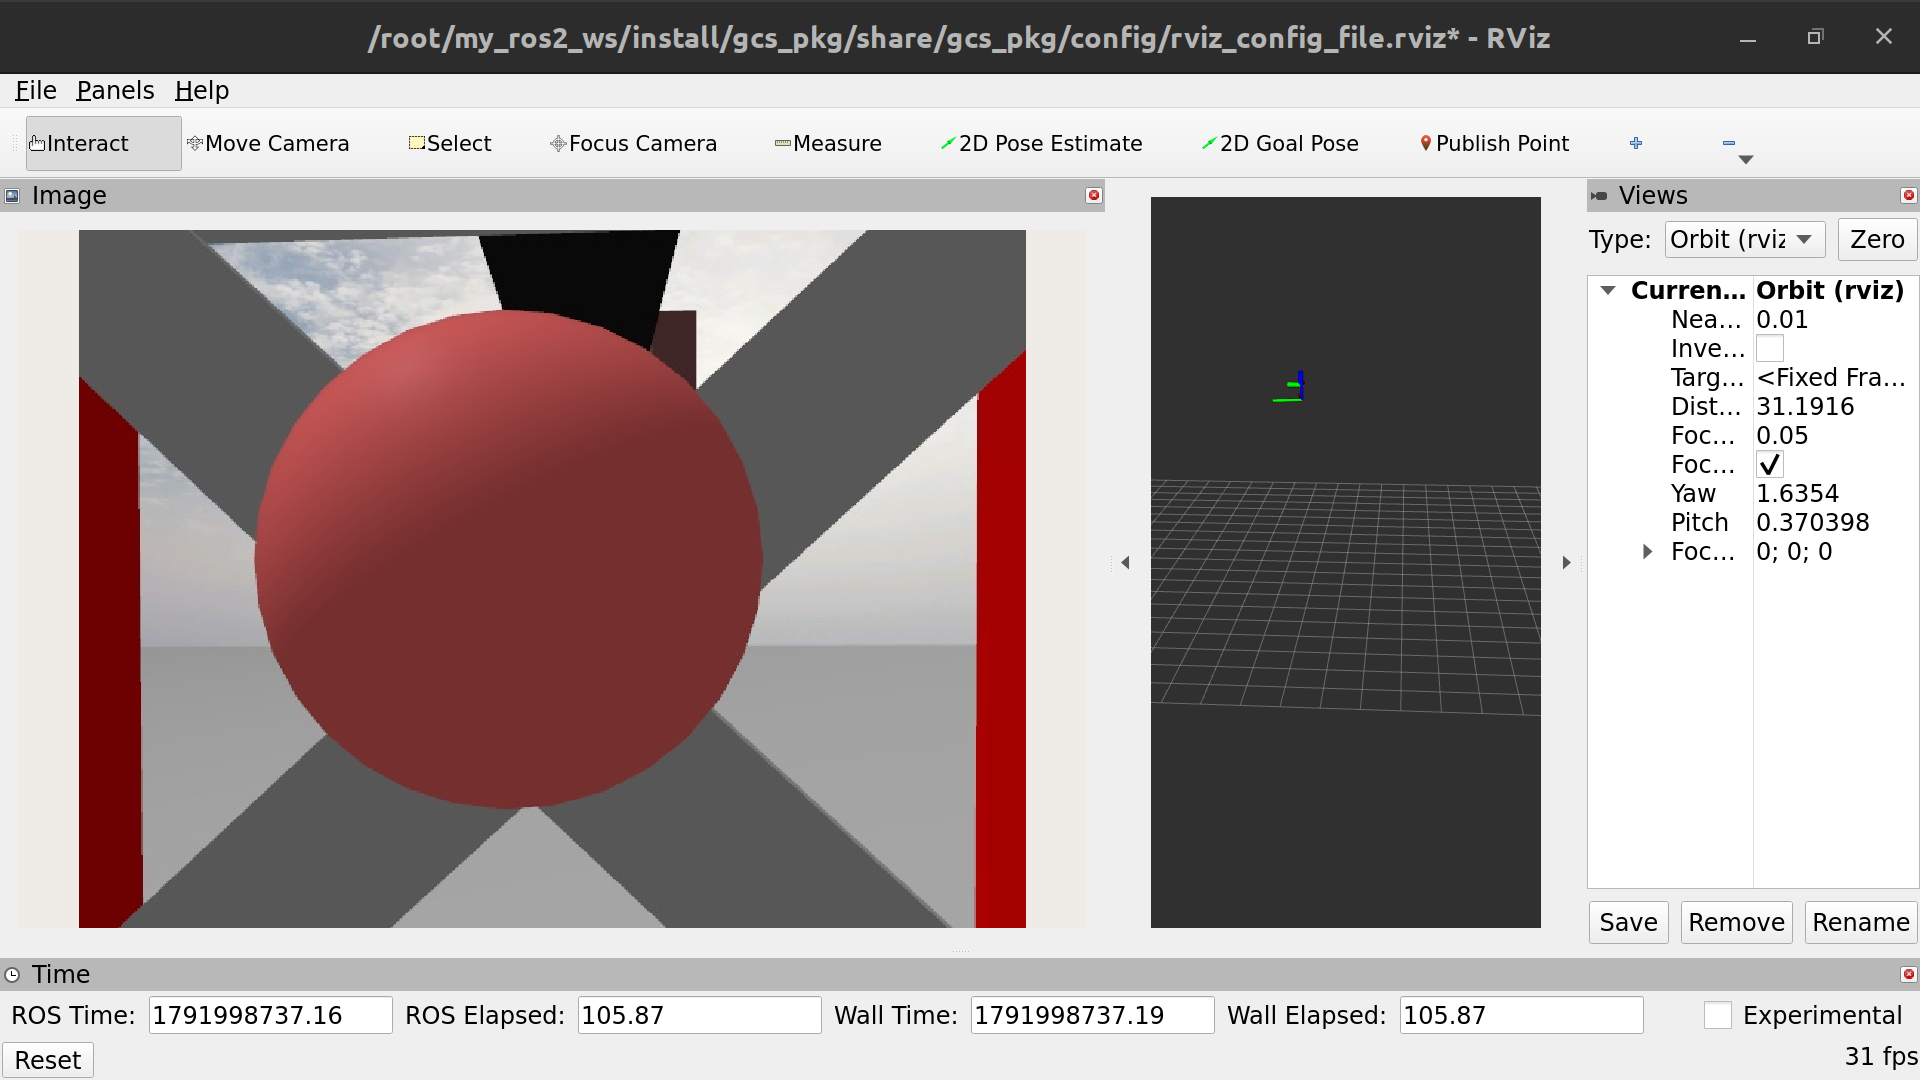
\includegraphics[width=\linewidth]{Immagini/Capitolo6/Simulations/PHASES/phase_obstacle.png}
    \caption{Navigation \& obstacle avoidance via teleoperation}
    \label{fig:sim_phase_obstacle}
\end{subfigure}
\hfill
\begin{subfigure}[b]{0.48\textwidth}
    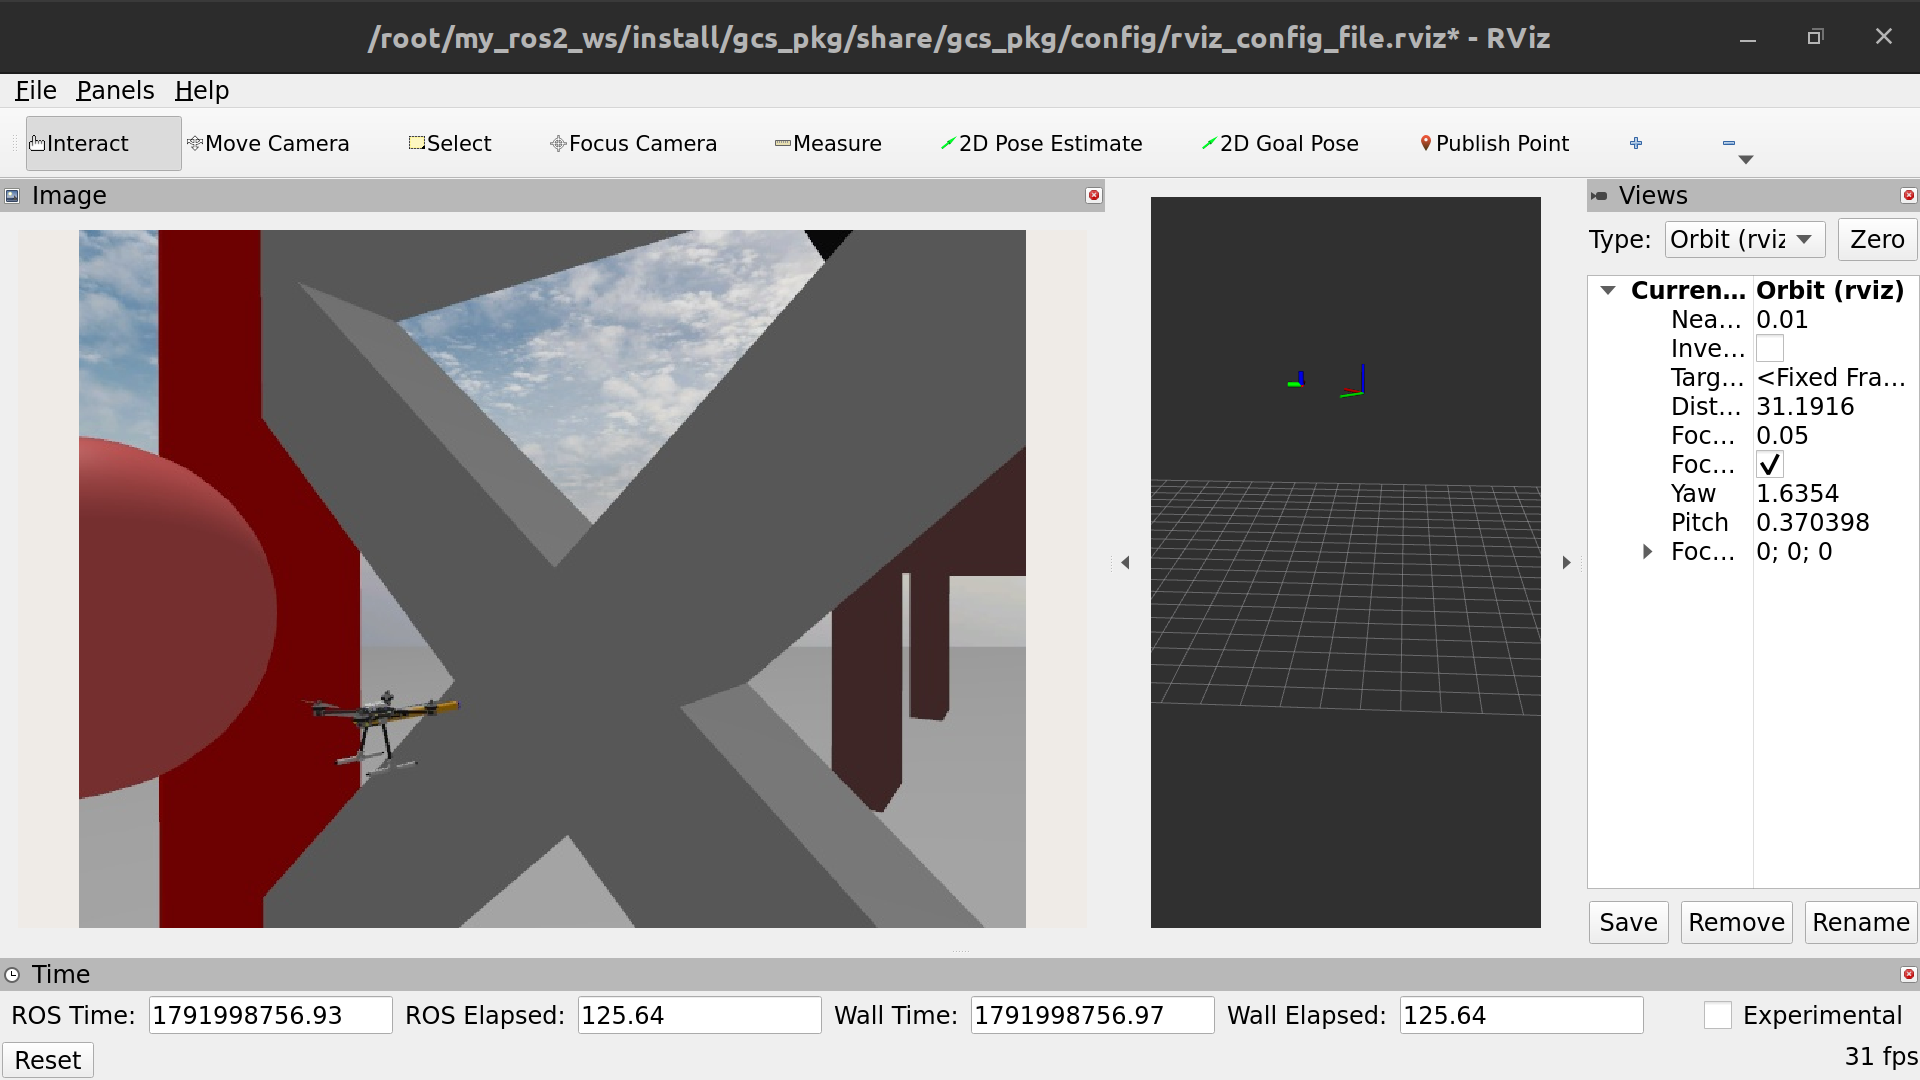
\includegraphics[width=\linewidth]{Immagini/Capitolo6/Simulations/PHASES/phase_approach.png}
    \caption{Autonomous approach toward target structure}
    \label{fig:sim_phase_approach}
\end{subfigure}
\\[1.5ex]
\begin{subfigure}[b]{0.48\textwidth}
    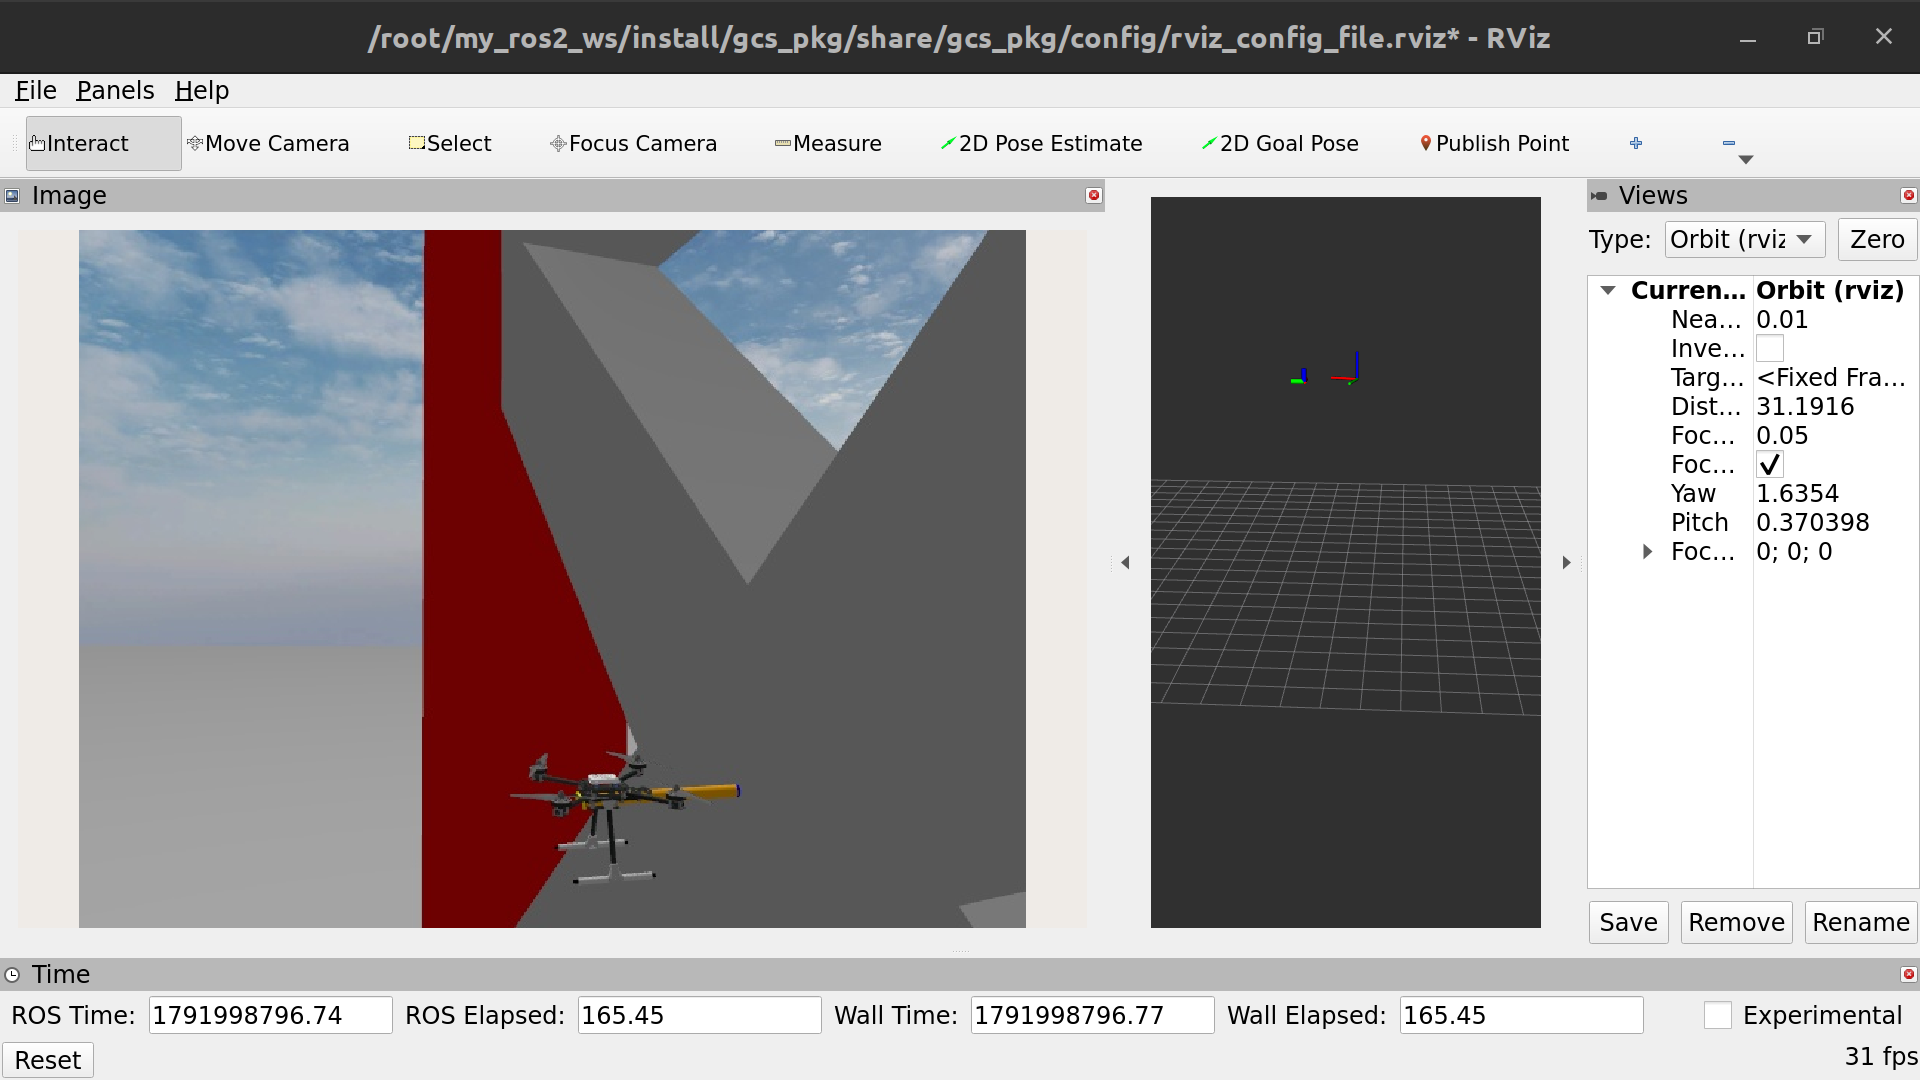
\includegraphics[width=\linewidth]{Immagini/Capitolo6/Simulations/PHASES/phase_interaction.png}
    \caption{Compliant physical contact and decoupled framing}
    \label{fig:sim_phase_interaction}
\end{subfigure}
\hfill
\begin{subfigure}[b]{0.48\textwidth}
    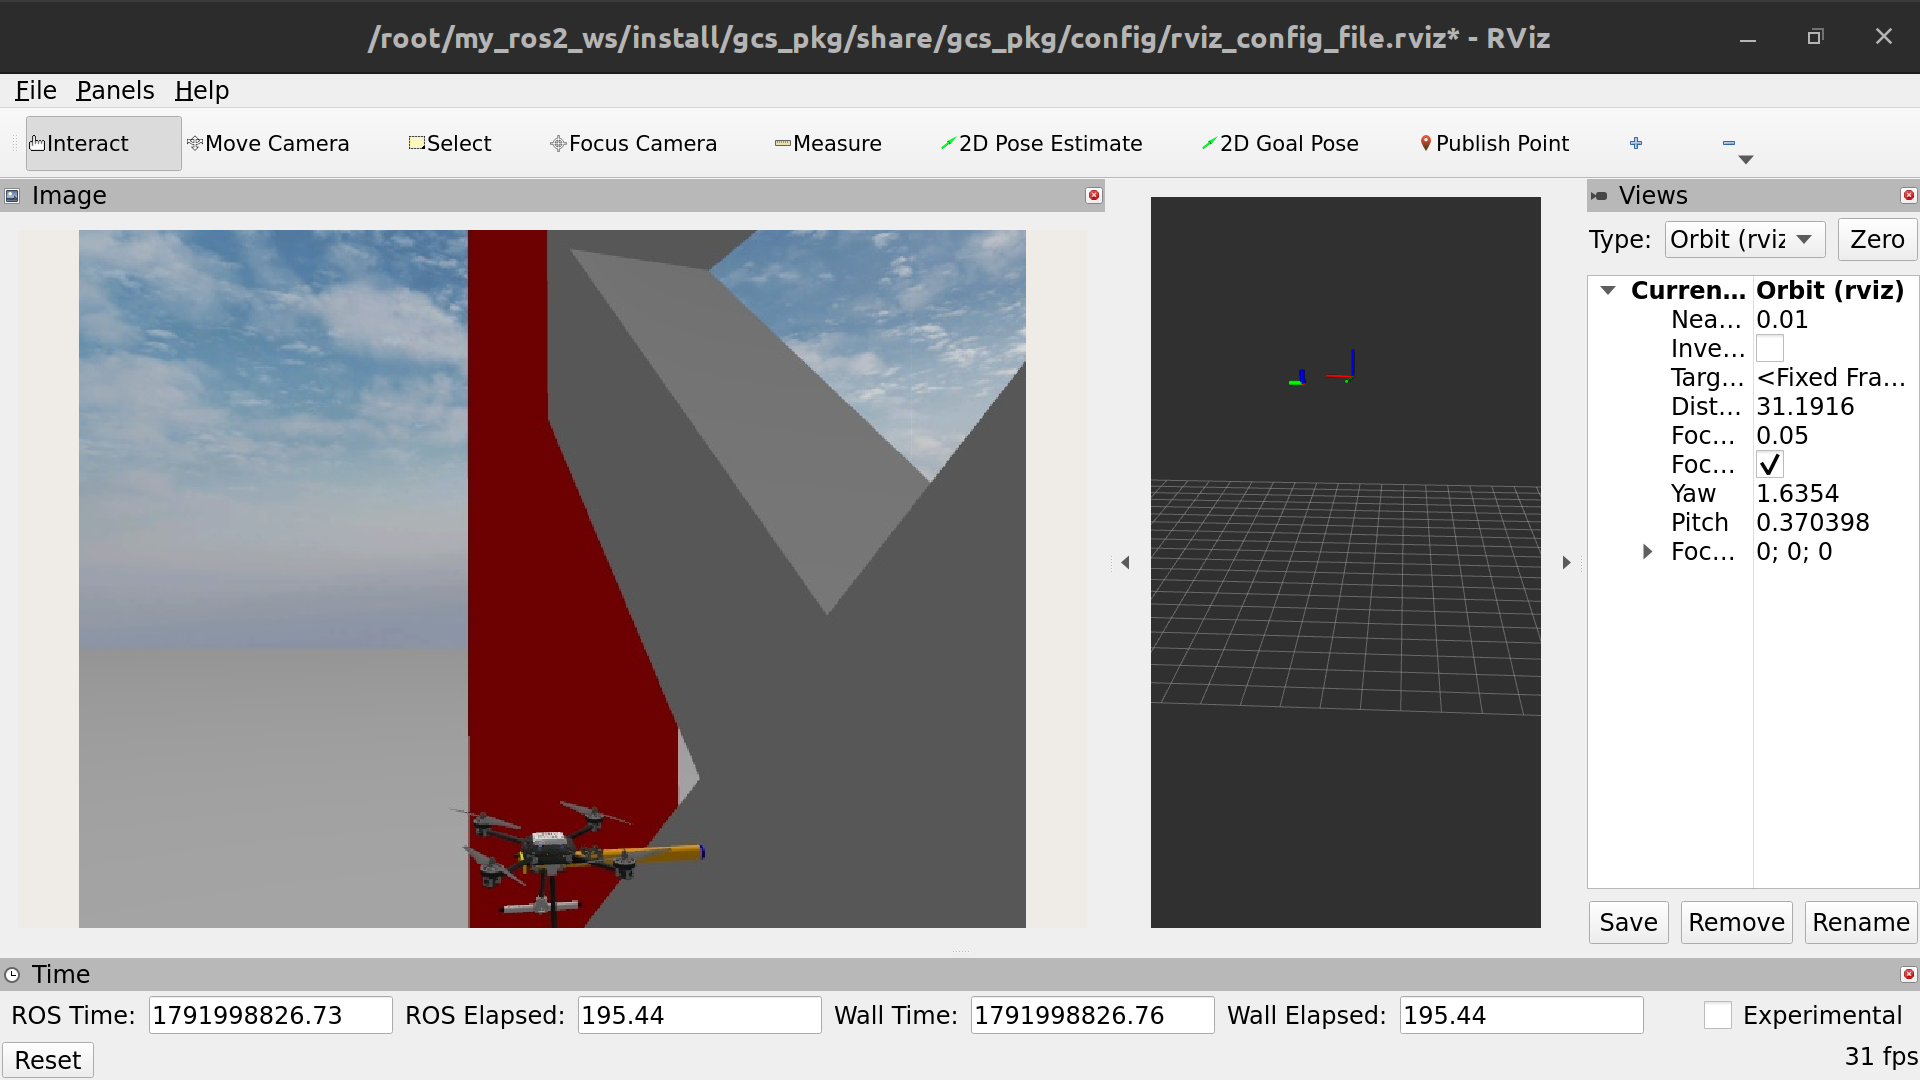
\includegraphics[width=\linewidth]{Immagini/Capitolo6/Simulations/PHASES/phase_detachment.png}
    \caption{Safe vehicle detachment}
    \label{fig:sim_phase_detachment}
\end{subfigure}
\\[1.5ex]
\begin{subfigure}[b]{0.50\textwidth}
    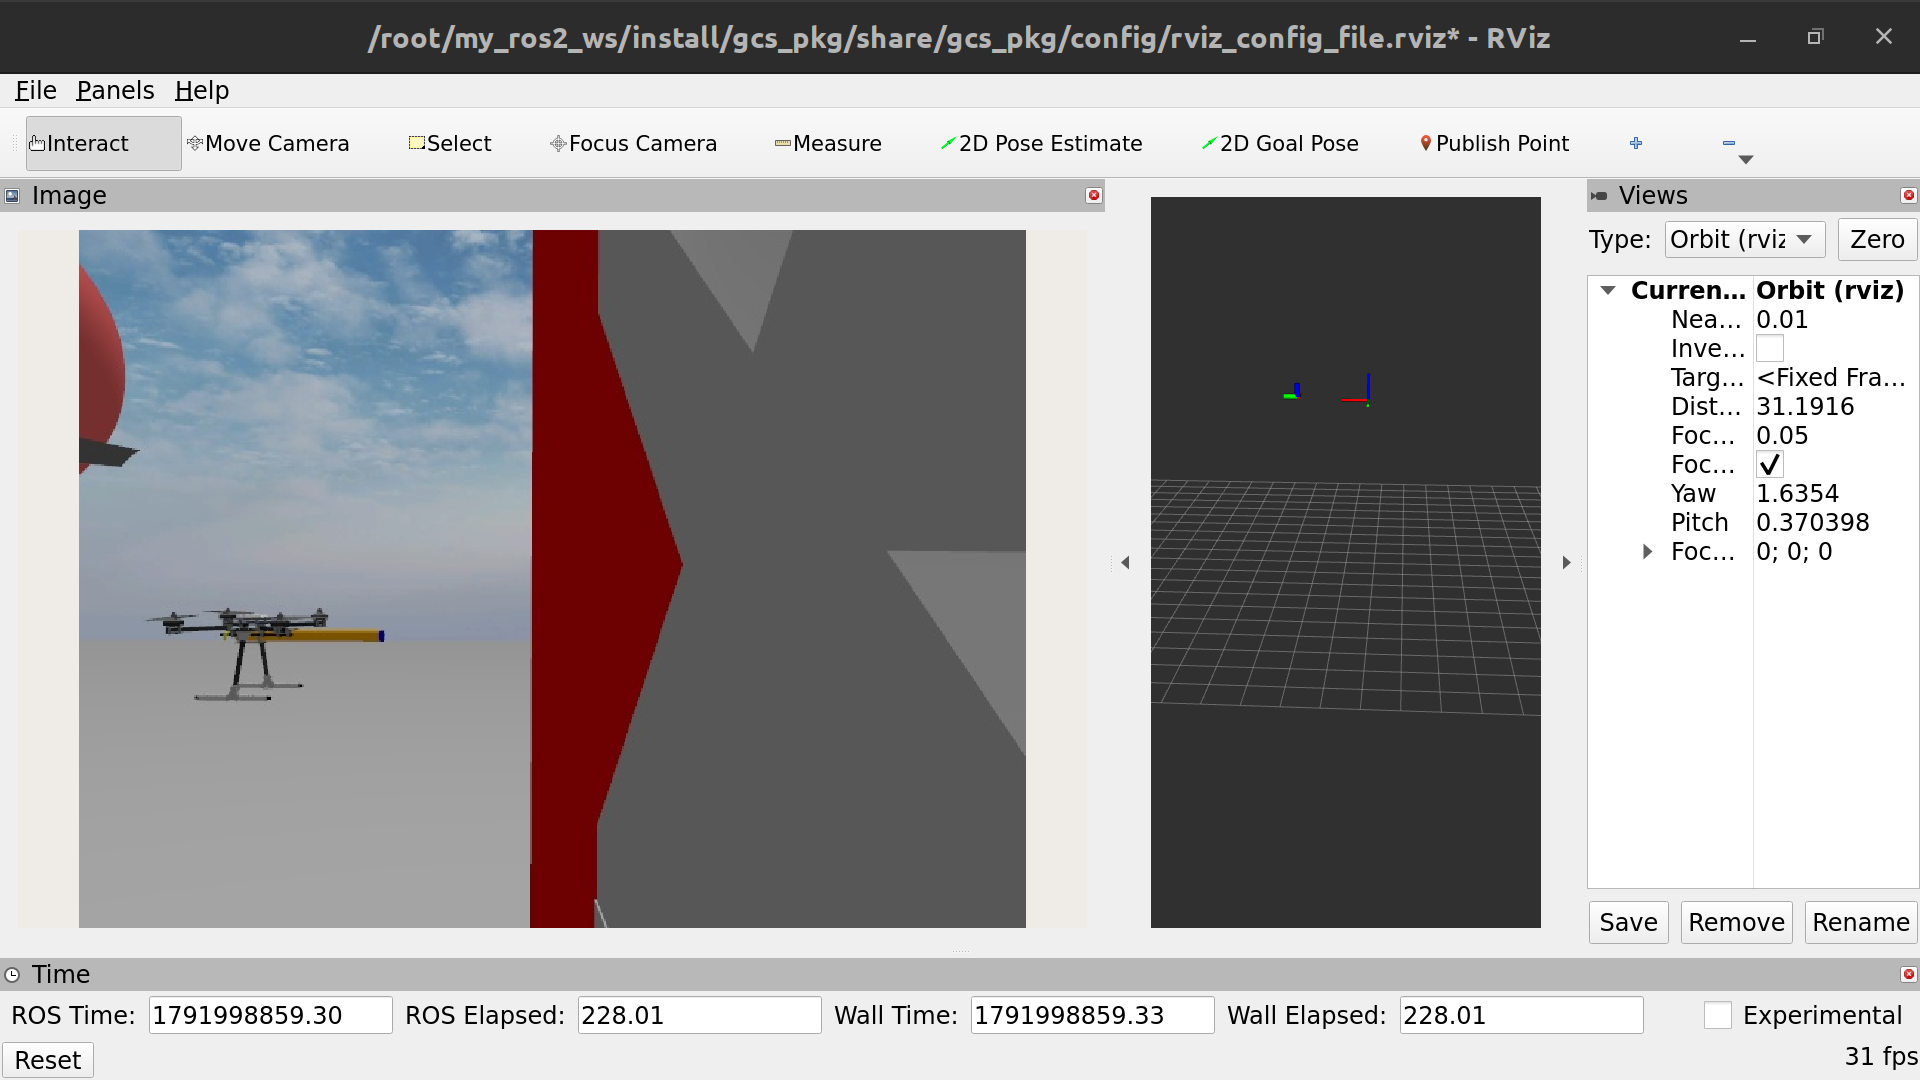
\includegraphics[width=\linewidth]{Immagini/Capitolo6/Simulations/PHASES/phase_return_home.png}
    \caption{Autonomous return-to-home navigation}
    \label{fig:sim_phase_return_home}
\end{subfigure}
\caption{Gazebo simulation snapshots illustrating the sequential operational phases of the cooperative mission}
\label{fig:sim_mission_phases}
\end{figure}

\begin{itemize}
    \item \textbf{Takeoff \& Hovering Switch:} Both UAVs execute a vertical take-off using PX4 position control. Upon reaching hovering altitude, the Observer UAV switches to the NMPC controller, locking onto the Inspection UAV and maintaining the target centered in the image plane.
    \item \textbf{Navigation \& Obstacle Avoidance (Figure \ref{fig:sim_phase_obstacle}):} During the transit toward the inspection area, an unmodeled spherical obstacle (highlighted in red) is placed along the Observer's flight corridor. This demonstrates the key advantage of the shared teleoperation channel: the human pilot uses the haptic joystick to smoothly dodge the obstacle with intuitive lateral/vertical inputs, while the NMPC dynamically preserves visual tracking and distance constraints, preventing loss of visual contact.
    \item \textbf{Approach (Figure \ref{fig:sim_phase_approach}):} The Inspection Drone navigates toward the target structure, arresting its forward motion at a safe standoff distance of $2\text{ m}$ from the wall. The Observer tracks it autonomously, keeping a centered viewpoint at nominal standoff distance $r \approx 2.5\text{--}2.7\text{ m}$ to maximize depth perception.
    \item \textbf{Interaction (Figure \ref{fig:sim_phase_interaction}):} Upon operator authorization, the Inspection Drone pushes against the surface. The admittance control loop accommodates the contact force ($\simeq 2\text{ N}$ with compliant displacement of $\simeq 4\text{ cm}$). Simultaneously, the FSM commands an elevated viewpoint ($z_{rel} \approx 0.78\text{ m}$) with a yaw offset, shifting the target drone toward the bottom-right corner of the image plane so that the end-effector tip and the wall remain centered and unobstructed in the video stream.
    \item \textbf{Detachment (Figure \ref{fig:sim_phase_detachment}):} Once inspection is complete, the Inspection Drone retreats by $0.5\text{ m}$ from the wall. The Observer adjusts its vantage point ($r \approx 2.18\text{ m}$) to grant the operator clear visual feedback of the vehicle disengagement.
    \item \textbf{Return Home (Figure \ref{fig:sim_phase_return_home}):} The Inspection Drone navigates back to its initial take-off coordinates, while the Observer drone smoothly restores a centered visual perspective ($z_{rel} \to 0$, $r \approx 2.5\text{ m}$) until disarm and landing.
\end{itemize}
\begin{figure}[h!]
    \centering
    \begin{subfigure}[b]{0.71\textwidth}
        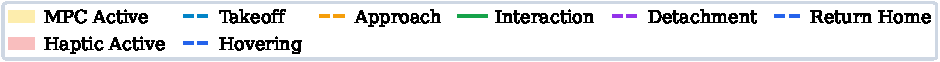
\includegraphics[width=\linewidth]{Immagini/Capitolo6/Simulations/Mission/phases_legend.pdf}
    \end{subfigure}
    \begin{subfigure}[b]{0.49\textwidth}
        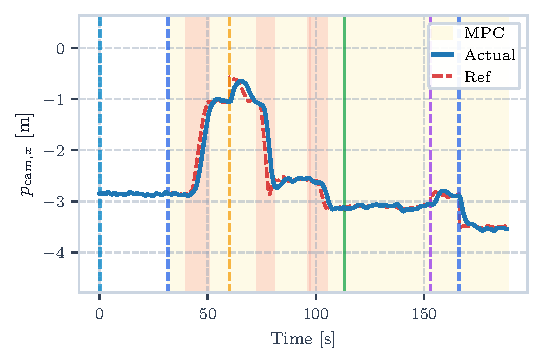
\includegraphics[width=\linewidth]{Immagini/Capitolo6/Simulations/Mission/POS_cam_x.pdf}
    \end{subfigure}
    \begin{subfigure}[b]{0.49\textwidth}
        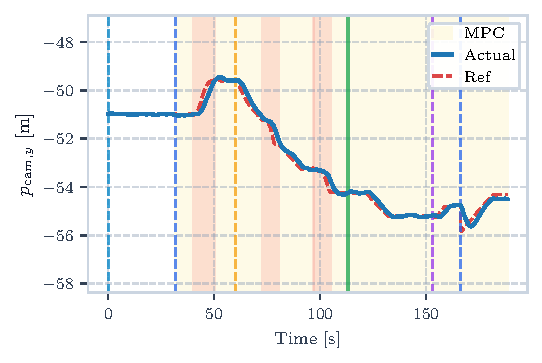
\includegraphics[width=\linewidth]{Immagini/Capitolo6/Simulations/Mission/POS_cam_y.pdf}
    \end{subfigure}
    \begin{subfigure}[b]{0.49\textwidth}
        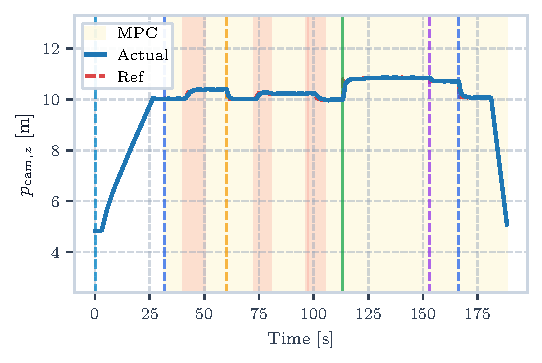
\includegraphics[width=\linewidth]{Immagini/Capitolo6/Simulations/Mission/POS_cam_z.pdf}
    \end{subfigure}
    \begin{subfigure}[b]{0.49\textwidth}
        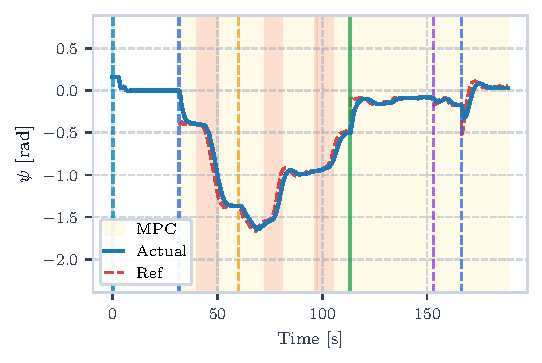
\includegraphics[width=\linewidth]{Immagini/Capitolo6/Simulations/Mission/YAW_yaw_actual_vs_desired.pdf}
    \end{subfigure}
    \caption{Position and orientation of the Observer Drone along the mission}
    \label{fig:mission_cam_pose}
\end{figure}
\begin{figure}[h!]
    \centering
    \begin{subfigure}[b]{0.71\textwidth}
        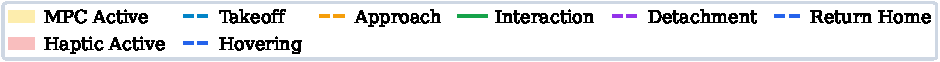
\includegraphics[width=\linewidth]{Immagini/Capitolo6/Simulations/Mission/phases_legend.pdf}
    \end{subfigure}
    \begin{subfigure}[b]{0.49\textwidth}
        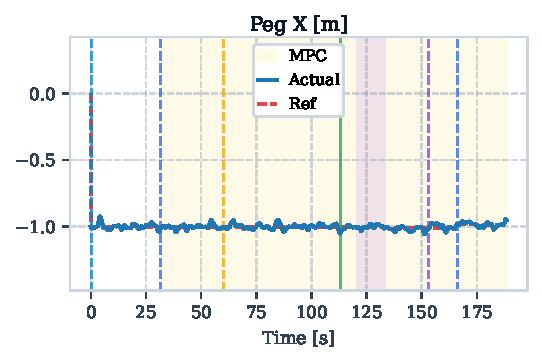
\includegraphics[width=\linewidth]{Immagini/Capitolo6/Simulations/Mission/INT_POS_peg_x.pdf}
    \end{subfigure}
    \begin{subfigure}[b]{0.49\textwidth}
        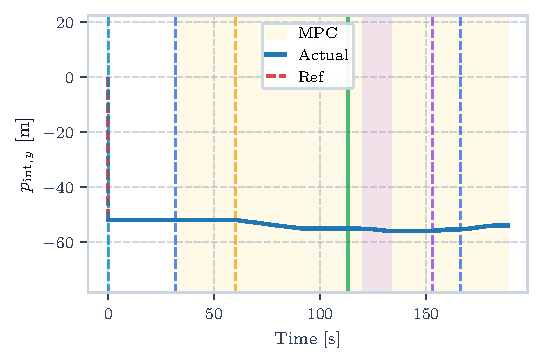
\includegraphics[width=\linewidth]{Immagini/Capitolo6/Simulations/Mission/INT_POS_peg_y.pdf}
    \end{subfigure}
    \begin{subfigure}[b]{0.49\textwidth}
        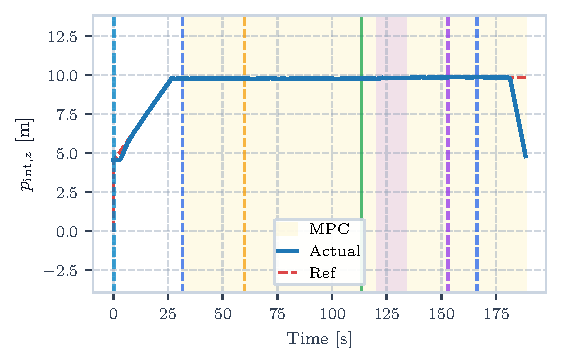
\includegraphics[width=\linewidth]{Immagini/Capitolo6/Simulations/Mission/INT_POS_peg_z.pdf}
    \end{subfigure}
    \begin{subfigure}[b]{0.49\textwidth}
        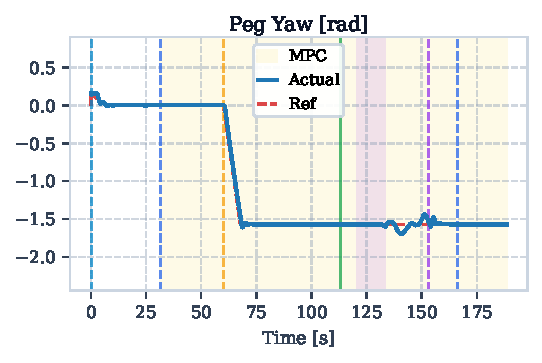
\includegraphics[width=\linewidth]{Immagini/Capitolo6/Simulations/Mission/INT_POS_peg_yaw.pdf}
    \end{subfigure}
    \caption{Position and orientation of the Interaction Drone along the mission}
    \label{fig:mission_int_pose}
\end{figure}
Figure \ref{fig:mission_cyl_pov} illustrates how the relative cylindrical variables are tracked across the mission and how relative setpoints adapt dynamically to each operational phase. During hovering and approach, the standoff distance is maintained around $r \approx 2.5\text{--}2.7\text{ m}$. During physical interaction, the reference adapts to $r_{\text{ref}} = 2.40\text{ m}$ to provide higher visual resolution of the contact interface, while the elevation offset increases to $z_{\text{rel}} \approx 0.78\text{ m}$ to frame the target vehicle in the lower corner of the field of view. During vehicle detachment, the radial distance contracts slightly to $r \approx 2.18\text{ m}$ to adapt the viewpoint before smoothly restoring the nominal distance $r \approx 2.50\text{ m}$ in the return-to-home phase.
\\Similarly, the elevation plot shows the autonomous offset introduced during interaction: by imposing an elevation displacement $z_{rel}$ and a corresponding yaw offset $\psi_{des}$, the target drone is deliberately shifted toward the bottom-right corner of the image plane. This ensures that the end-effector tip and the inspected wall remain fully visible and centered in the operator's FOV. The tracking errors across all cylindrical coordinates remain strictly bounded, proving that the NMPC smoothly handles the reference discontinuities commanded by the FSM without inducing aggressive transients or video shake.
\begin{figure}[h!]
\centering
\begin{subfigure}[b]{0.71\textwidth}
    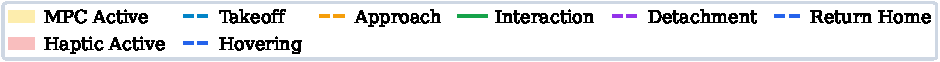
\includegraphics[width=\linewidth]{Immagini/Capitolo6/Simulations/Mission/phases_legend.pdf}
\end{subfigure}
\begin{subfigure}[b]{0.49\textwidth}
    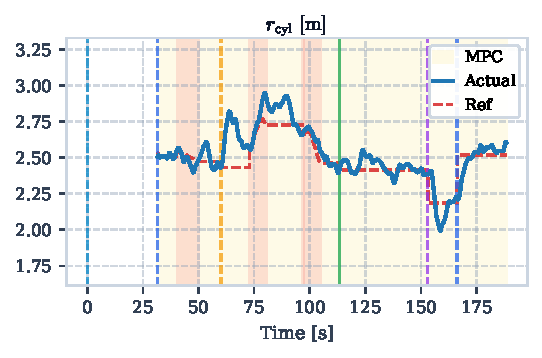
\includegraphics[width=\linewidth]{Immagini/Capitolo6/Simulations/Mission/CYL_POV_distance_r_cyl.pdf}
\end{subfigure}
\begin{subfigure}[b]{0.49\textwidth}
    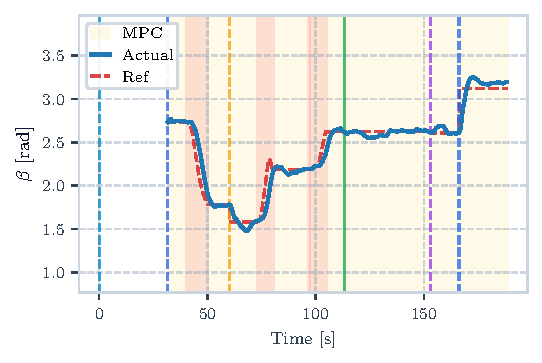
\includegraphics[width=\linewidth]{Immagini/Capitolo6/Simulations/Mission/CYL_POV_azimuth_beta.pdf}
\end{subfigure}
\begin{subfigure}[b]{0.49\textwidth}
    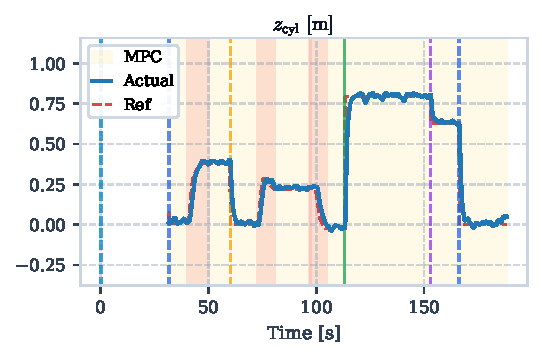
\includegraphics[width=\linewidth]{Immagini/Capitolo6/Simulations/Mission/CYL_POV_elevation_z.pdf}
\end{subfigure}
\begin{subfigure}[b]{0.49\textwidth}
    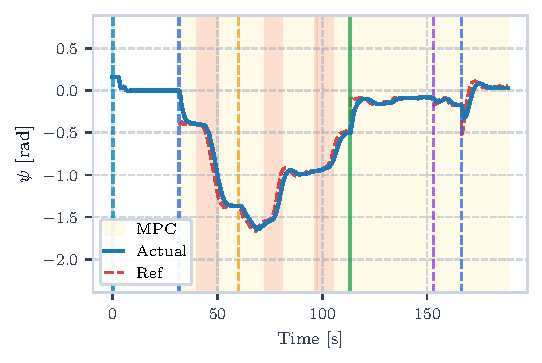
\includegraphics[width=\linewidth]{Immagini/Capitolo6/Simulations/Mission/YAW_yaw_actual_vs_desired.pdf}
\end{subfigure}
\caption{Cylindrical visual tracking variables along the cooperative mission}
\label{fig:mission_cyl_pov}
\end{figure}
To prevent visual fatigue and motion sickness for the operator, the NMPC formulation explicitly minimizes higher-order dynamic derivatives in the cost function. Figure \ref{fig:mission_derivative_norms} reports the Euclidean norms of linear acceleration, angular acceleration, jerk, and snap along the entire mission. 
\\As shown in the plots, all derivative norms remain smooth and bounded throughout the flight. Small variations occur only during phase transitions when adapting to new visual setpoints, but high-frequency jerk and snap are heavily damped. This validates that the camera motion remains remarkably fluid and free of sharp shakes, keeping the streamed video comfortable for human decision-making.
\begin{figure}[h!]
\centering
\begin{subfigure}[b]{0.71\textwidth}
    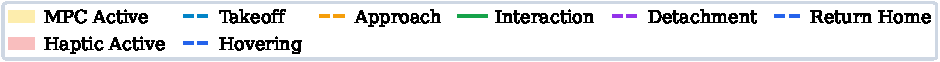
\includegraphics[width=\linewidth]{Immagini/Capitolo6/Simulations/Mission/phases_legend.pdf}
\end{subfigure}
\begin{subfigure}[b]{0.49\textwidth}
    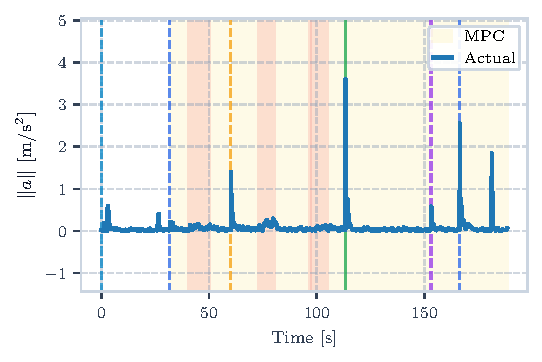
\includegraphics[width=\linewidth]{Immagini/Capitolo6/Simulations/Mission/DERIVATIVE_NORMS_norm_acc.pdf}
\end{subfigure}
\begin{subfigure}[b]{0.49\textwidth}
    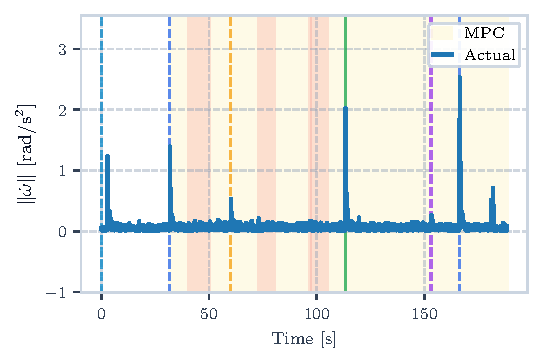
\includegraphics[width=\linewidth]{Immagini/Capitolo6/Simulations/Mission/DERIVATIVE_NORMS_norm_angacc.pdf}
\end{subfigure}
\begin{subfigure}[b]{0.49\textwidth}
    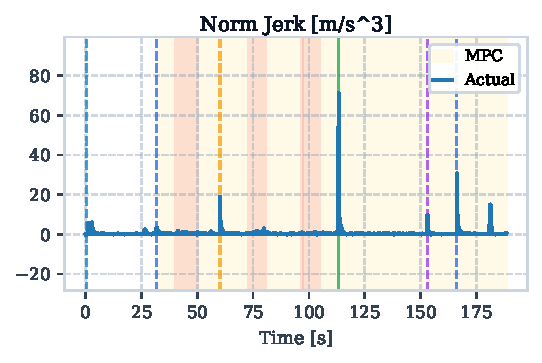
\includegraphics[width=\linewidth]{Immagini/Capitolo6/Simulations/Mission/DERIVATIVE_NORMS_norm_jerk.pdf}
\end{subfigure}
\begin{subfigure}[b]{0.49\textwidth}
    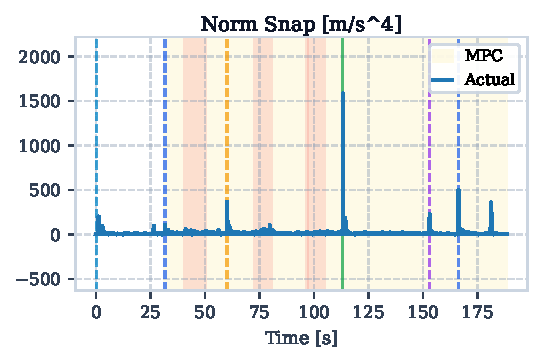
\includegraphics[width=\linewidth]{Immagini/Capitolo6/Simulations/Mission/DERIVATIVE_NORMS_norm_snap.pdf}
\end{subfigure}
\caption{Norms of higher-order dynamic derivatives penalised in the NMPC cost function during the mission}
\label{fig:mission_derivative_norms}
\end{figure}
Since the NMPC acts directly as a low-level dynamic controller, Figure \ref{fig:mission_control_wrench} illustrates the actual control wrench commanded to the Observer UAV. The total thrust $F_z$ stays around the nominal hovering weight ($\simeq 14.7\text{ N}$) without dangerous drops during the maneuvers. The commanded body torques ($\tau_x, \tau_y, \tau_z$) remain smooth and strictly inside the hard actuation bounds enforced by the solver ($[-U_\tau, U_\tau]$). Similar to the hovering test, $\tau_y$ compensates for the unmodeled camera offset without creating any instability, demonstrating the effectiveness of the online MBE feedforward.
\begin{figure}[h!]
\centering
\begin{subfigure}[b]{0.71\textwidth}
    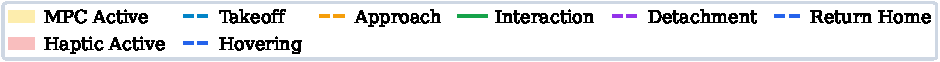
\includegraphics[width=\linewidth]{Immagini/Capitolo6/Simulations/Mission/phases_legend.pdf}
\end{subfigure}
\begin{subfigure}[b]{0.49\textwidth}
    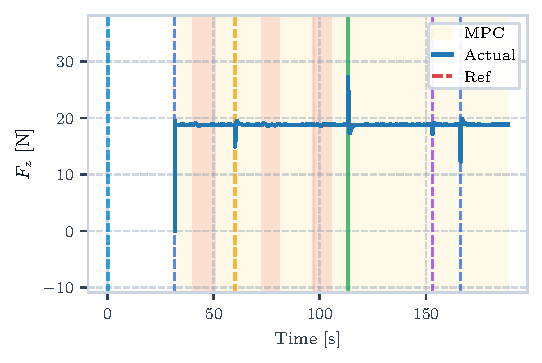
\includegraphics[width=\linewidth]{Immagini/Capitolo6/Simulations/Mission/CONTROL_WRENCH_force_z.pdf}
\end{subfigure}
\begin{subfigure}[b]{0.49\textwidth}
    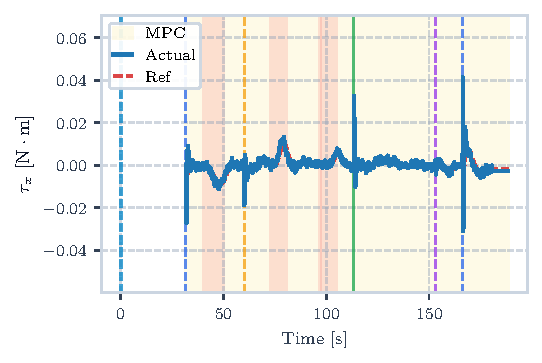
\includegraphics[width=\linewidth]{Immagini/Capitolo6/Simulations/Mission/CONTROL_WRENCH_torque_x.pdf}
\end{subfigure}
\begin{subfigure}[b]{0.49\textwidth}
    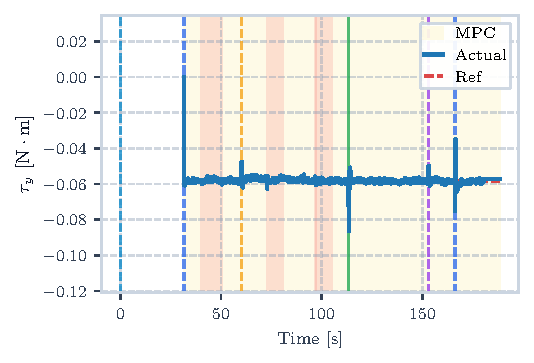
\includegraphics[width=\linewidth]{Immagini/Capitolo6/Simulations/Mission/CONTROL_WRENCH_torque_y.pdf}
\end{subfigure}
\begin{subfigure}[b]{0.49\textwidth}
    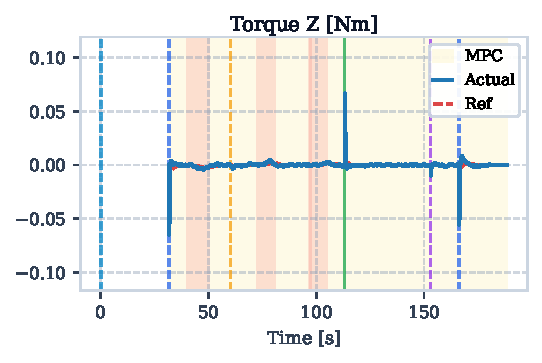
\includegraphics[width=\linewidth]{Immagini/Capitolo6/Simulations/Mission/CONTROL_WRENCH_torque_z.pdf}
\end{subfigure}
\caption{Control wrench commanded by the NMPC to the Observer UAV along the mission}
\label{fig:mission_control_wrench}
\end{figure}
A critical phase of this mission is the physical interaction with the environment. When the Inspection Drone touches the target surface, the tip-mounted virtual 1D force sensor detects the collision. 
\begin{figure}[h!]
    \centering
    \begin{subfigure}[b]{0.6\textwidth}
        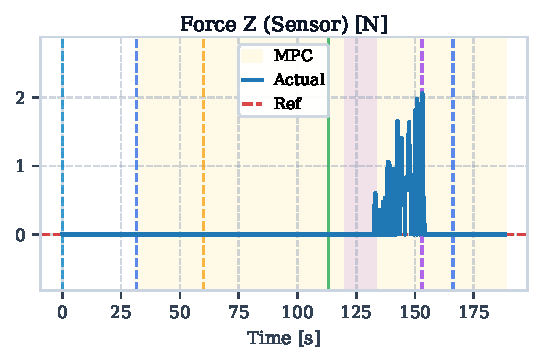
\includegraphics[width=\linewidth]{Immagini/Capitolo6/Simulations/Mission/SENSOR_FORCES_force_z.pdf}    
    \end{subfigure}
    \begin{subfigure}[b]{0.6\textwidth}
        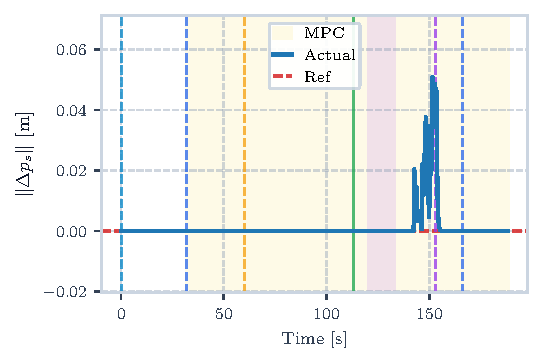
\includegraphics[width=\linewidth]{Immagini/Capitolo6/Simulations/Mission/INT_ADMITTANCE_SENSOR_p_s.pdf}
    \end{subfigure}
    \caption{Pre-filtered contact force and admittance displacement norm in sensor frame}
    \label{fig:admittance}
\end{figure}
As illustrated in Figure \ref{fig:admittance}, the raw contact forces are successfully filtered and processed by the admittance node. The bottom half of the plot highlights the deviation between the nominal, rigid trajectory and the compliant reference generated by the mass-damper-spring model given by admittance filter. Consequently, the Inspection Drone smoothly accommodates the external force, preventing mechanical damage and ensuring a safe and stable contact phase. A displacement of $\simeq4$cm is estimated by the filter, correspondent to $2$N external force.
\\Moreover, thanks to the dynamic behavior of the NMPC, the Observer Drone compensates for this sudden compliant shift of its target. The visual tracking remains robust throughout the entire interaction, validating the performance of the proposed multi-drone framework.

\section{Preliminary Real-World Experimental Assessment}
\textcolor{red}{***AGGIUNGERE SEQUENZE SCREENSHOTS ESPERIMENTO REALE***}
\\To validate the transition from simulation to real hardware, preliminary flight tests were carried out focusing on the Observer UAV tracking an independent target vehicle. 
As detailed in previous chapters, the physical Observer UAV is a custom octocopter platform running the full NMPC pipeline directly onboard a LattePanda companion computer at $100\text{ Hz}$, interfaced with a Pixhawk 4 flight controller running PX4 via Micro-XRCE-DDS over serial. A manually piloted quadrotor acts as the physical visual target.
\\One of the objectives was to verify the real-time execution of the embedded solver and evaluate tracking robustness in the presence of real aerodynamics, sensor noise, and communication delays.
\begin{figure}[h!]
\centering
\begin{subfigure}[b]{0.71\textwidth}
    
\includegraphics[width=\linewidth]{Immagini/Capitolo6/Experiments/phases_legend.pdf}
\end{subfigure}
\begin{subfigure}[b]{0.49\textwidth}
    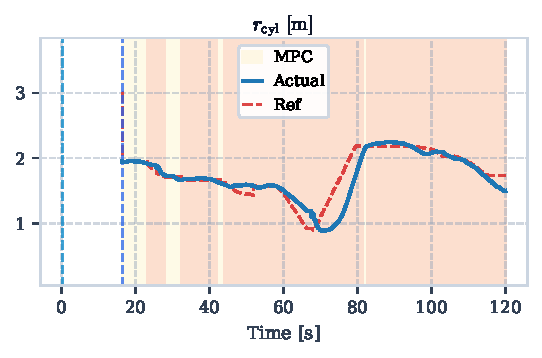
\includegraphics[width=\linewidth]{Immagini/Capitolo6/Experiments/CYL_POV_distance_r_cyl.pdf}
\end{subfigure}
\begin{subfigure}[b]{0.49\textwidth}
    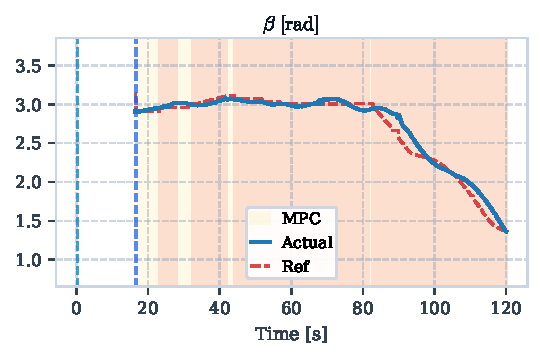
\includegraphics[width=\linewidth]{Immagini/Capitolo6/Experiments/CYL_POV_azimuth_beta.pdf}
\end{subfigure}
\begin{subfigure}[b]{0.49\textwidth}
    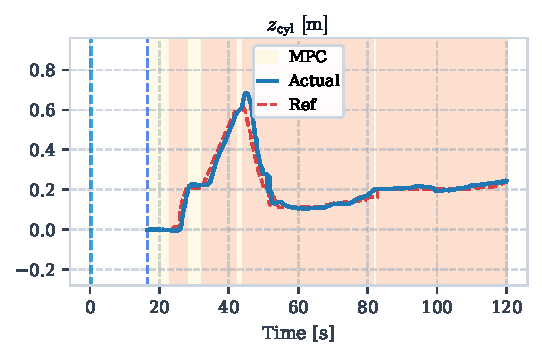
\includegraphics[width=\linewidth]{Immagini/Capitolo6/Experiments/CYL_POV_elevation_z.pdf}
\end{subfigure}
\begin{subfigure}[b]{0.49\textwidth}
    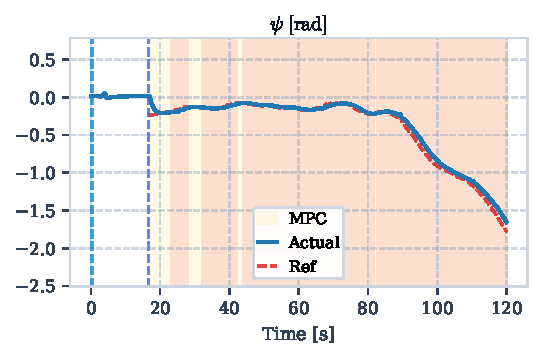
\includegraphics[width=\linewidth]{Immagini/Capitolo6/Experiments/YAW_yaw_actual_vs_desired.pdf}
\end{subfigure}
\caption{Cylindrical visual tracking variables along the real-world flight test}
\label{fig:hw_cyl_pov}
\end{figure}
The tracking performance in relative cylindrical coordinates is reported in Figure \ref{fig:hw_cyl_pov}. Despite the aerodynamic disturbances, the vehicle maintains the relative standoff distance with an RMS error of $0.18\text{ m}$, and controls elevation with high precision (RMS error of $3.1\text{ cm}$). The yaw orientation follows the relative azimuth smoothly, keeping the target centered in the camera frame with an RMS error of $3.07^\circ$.
\begin{figure}[h!]
\centering
\begin{subfigure}[b]{0.51\textwidth}
    
\includegraphics[width=\linewidth]{Immagini/Capitolo6/Experiments/phases_legend.pdf}
\end{subfigure}
\begin{subfigure}[b]{0.8\textwidth}
    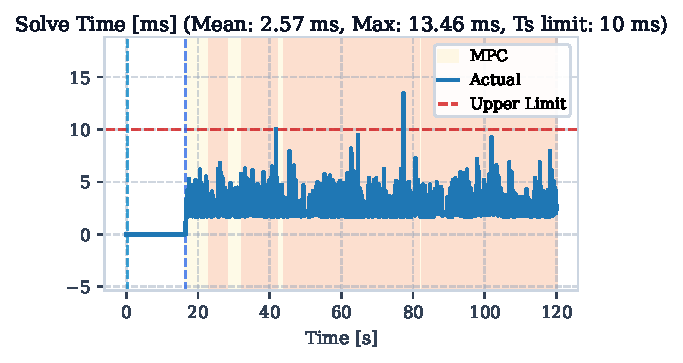
\includegraphics[width=\linewidth]{Immagini/Capitolo6/Experiments/SOLVE_TIME_solve_time.pdf}
\end{subfigure}
\caption{Onboard NMPC solving time on the LattePanda companion computer during experimental flight}
\label{fig:hw_solve_time}
\end{figure}
Figure \ref{fig:hw_solve_time} reports the execution time of the NMPC solver executed onboard the LattePanda computer throughout the flight. The solver demonstrates high computational efficiency: the mean execution time is $2.57\text{ ms}$, corresponding to an average CPU load of only $25.7\%$ within the $10\text{ ms}$ control step ($100\text{ Hz}$). The 99th percentile reaches $6.25\text{ ms}$, with solver overruns ($>10\text{ ms}$) limited to $0.08\%$ ($2$ cycles over $2649$), fully absorbed by the real-time iteration (SQP-RTI) scheme without inducing instability.

\begin{figure}[h!]
\centering
\begin{subfigure}[b]{0.51\textwidth}
    
\includegraphics[width=\linewidth]{Immagini/Capitolo6/Experiments/phases_legend.pdf}
\end{subfigure}
\begin{subfigure}[b]{0.8\textwidth}
    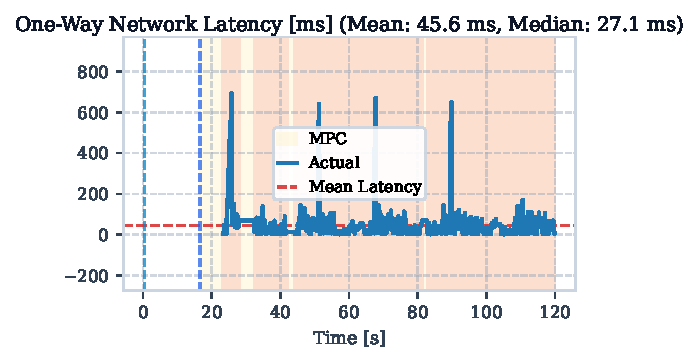
\includegraphics[width=\linewidth]{Immagini/Capitolo6/Experiments/HAPTIC_LATENCY_latency.pdf}
\end{subfigure}
\caption{One-way network communication latency of the bilateral haptic teleoperation channel during physical flight}
\label{fig:hw_haptic_latency}
\end{figure}
To assess the communication performance of the shared teleoperation loop over the local wireless link, Figure \ref{fig:hw_haptic_latency} reports the one-way network latency between the Ground Control Station (interfaced with the Novint Falcon) and the onboard companion computer. During active teleoperation phases (highlighted by the red shaded regions), the mean one-way latency is $45.56\text{ ms}$, with a median of $27.14\text{ ms}$ and a 95th percentile contained within $92.90\text{ ms}$. This latency profile satisfies standard haptic transparency requirements, allowing the human operator to receive responsive tactile feedback without inducing delay-driven instabilities.

To verify camera stability and the absence of high-frequency shakes during physical flight, Figure \ref{fig:hw_derivative_norms} reports the Euclidean norms of linear acceleration, angular acceleration, jerk, and snap recorded onboard.
\begin{figure}[h!]
\centering
\begin{subfigure}[b]{0.71\textwidth}
    
\includegraphics[width=\linewidth]{Immagini/Capitolo6/Experiments/phases_legend.pdf}
\end{subfigure}
\begin{subfigure}[b]{0.49\textwidth}
    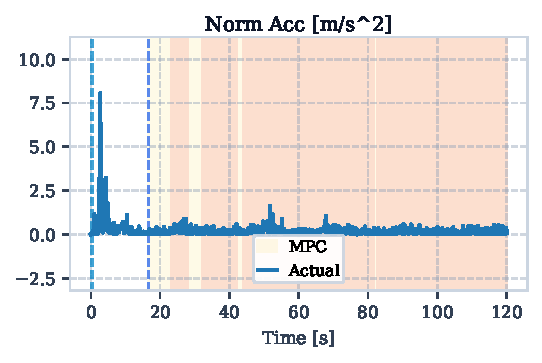
\includegraphics[width=\linewidth]{Immagini/Capitolo6/Experiments/DERIVATIVE_NORMS_norm_acc.pdf}
\end{subfigure}
\begin{subfigure}[b]{0.49\textwidth}
    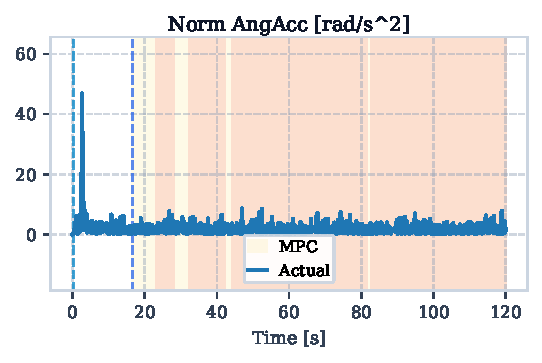
\includegraphics[width=\linewidth]{Immagini/Capitolo6/Experiments/DERIVATIVE_NORMS_norm_angacc.pdf}
\end{subfigure}
\begin{subfigure}[b]{0.49\textwidth}
    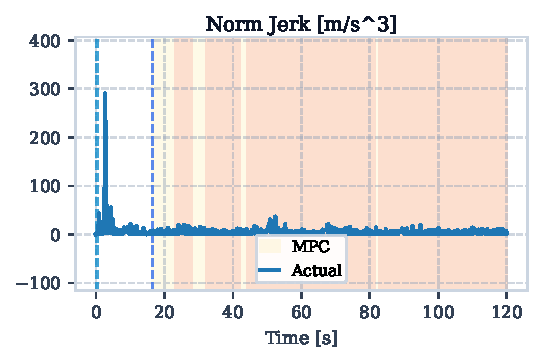
\includegraphics[width=\linewidth]{Immagini/Capitolo6/Experiments/DERIVATIVE_NORMS_norm_jerk.pdf}
\end{subfigure}
\begin{subfigure}[b]{0.49\textwidth}
    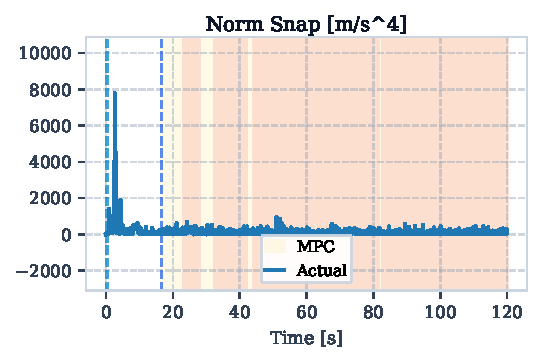
\includegraphics[width=\linewidth]{Immagini/Capitolo6/Experiments/DERIVATIVE_NORMS_norm_snap.pdf}
\end{subfigure}
\caption{Norms of higher-order dynamic derivatives penalised in the NMPC cost function during real-world flight}
\label{fig:hw_derivative_norms}
\end{figure}
As highlighted by the plots, the higher derivative norms remain strictly bounded throughout the test. Even under aerodynamical downwash and target speed changes, the high-frequency jerk and snap components are strongly penalized by the NMPC cost function, preventing jerky camera motions and potential motion sickness for the human operator.

\begin{figure}[h!]
\centering
\begin{subfigure}[b]{0.71\textwidth}
    
\includegraphics[width=\linewidth]{Immagini/Capitolo6/Experiments/phases_legend.pdf}
\end{subfigure}
\begin{subfigure}[b]{0.32\textwidth}
    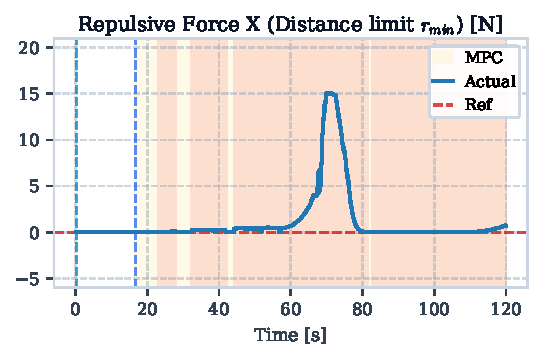
\includegraphics[width=\linewidth]{Immagini/Capitolo6/Experiments/REPULSIVE_FORCES_repulsive_force_x.pdf}
\end{subfigure}
\begin{subfigure}[b]{0.32\textwidth}
    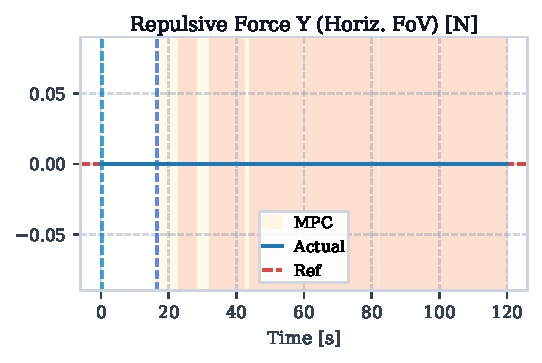
\includegraphics[width=\linewidth]{Immagini/Capitolo6/Experiments/REPULSIVE_FORCES_repulsive_force_y.pdf}
\end{subfigure}
\begin{subfigure}[b]{0.32\textwidth}
    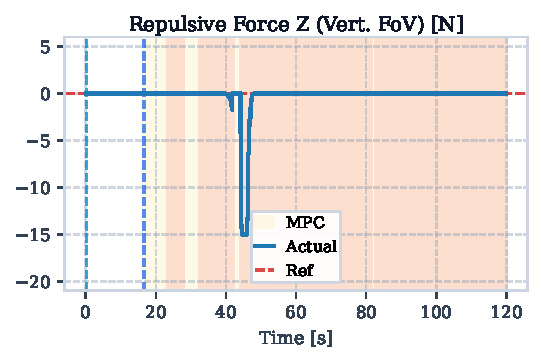
\includegraphics[width=\linewidth]{Immagini/Capitolo6/Experiments/REPULSIVE_FORCES_repulsive_force_z.pdf}
\end{subfigure}
\caption{Artificial potential field repulsive forces transmitted to the Novint Falcon haptic joystick during real-world flight}
\label{fig:hw_haptic_rep}
\end{figure}

\begin{figure}[h!]
\centering
\begin{subfigure}[b]{0.71\textwidth}
    
\includegraphics[width=\linewidth]{Immagini/Capitolo6/Experiments/phases_legend.pdf}
\end{subfigure}
\begin{subfigure}[b]{0.32\textwidth}
    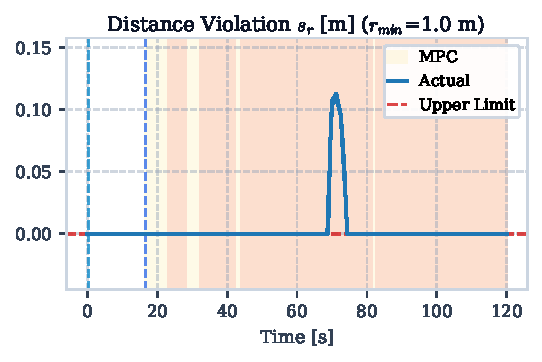
\includegraphics[width=\linewidth]{Immagini/Capitolo6/Experiments/APF_distance_violation_s_r.pdf}
\end{subfigure}
\begin{subfigure}[b]{0.32\textwidth}
    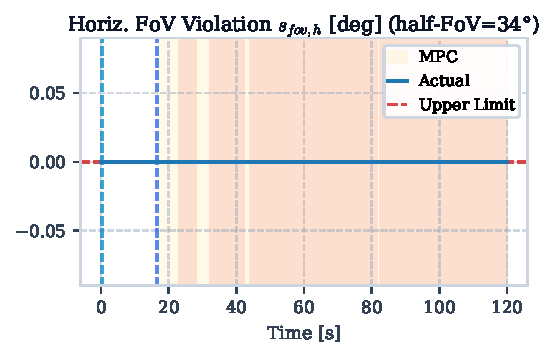
\includegraphics[width=\linewidth]{Immagini/Capitolo6/Experiments/APF_horiz_fov_violation_s__fov_h.pdf}
\end{subfigure}
\begin{subfigure}[b]{0.32\textwidth}
    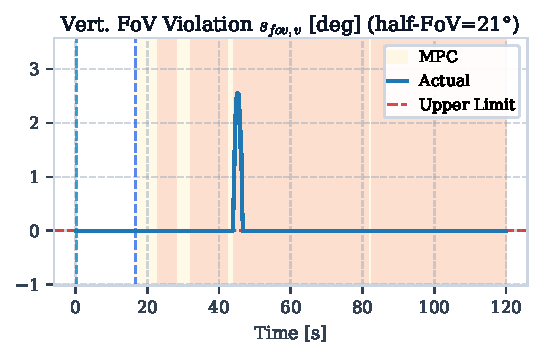
\includegraphics[width=\linewidth]{Immagini/Capitolo6/Experiments/APF_vert_fov_violation_s__fov_v.pdf}
\end{subfigure}
\caption{Safety distance and camera Field of View constraint violations during experimental flight}
\label{fig:hw_apf_violations}
\end{figure}

Figures \ref{fig:hw_haptic_rep} and \ref{fig:hw_apf_violations} illustrate the bilateral interaction between the human operator and the aerial platform through the Novint Falcon haptic interface. In our shared control formulation, the artificial potential field acts as an anticipatory safety barrier: when human teleoperation commands the vehicle towards an unfeasible configuration, exponential repulsive forces push the control handle back.
\\Specifically, during radial teleoperation around $t \approx 70\text{ s}$, the pilot pushes the joystick forward to inspect the target at close range. As the inter-drones distance approaches the safety boundary $r_{\min} = 1.0\text{ m}$ (with a transient encroachment peaking at $s_r = 0.11\text{ m}$), the repulsive force $F_x^{\text{rep}}$ rises steeply and reaches the physical saturation threshold of $15.0\text{ N}$. The strong tactile resistance informs the operator of the impending collision hazard, leading them to ease the forward pressure. As a result, the distance smoothly recovers beyond $1.5\text{ m}$, and $s_r$ promptly returns to zero.
\\A similar protective behavior occurs along the vertical direction around $t \approx 45\text{ s}$. When the operator commands an upward climb, bringing the target close to the upper limit of the vertical camera Field of View ($\text{FOV}_v = 42^\circ$, corresponding to a semi-aperture of $21^\circ$), the target slightly exceeds the viewing boundary ($s_{fov,v} = 2.56^\circ$). In response, the APF exerts a peak downward force $F_z^{\text{rep}} = -15.0\text{ N}$, saturated to $10 \text{N}$, on the joystick, prompting the human operator to lower the setpoint and immediately re-centering the target within the camera frame ($s_{fov,v} \to 0$).
\\Along the horizontal direction, because the autonomous yaw tracking loop maintains the optical axis tightly aligned with the target ($|\psi_{\text{err}}| \le 16.5^\circ$, well within the horizontal semi-aperture of $34.5^\circ$), the horizontal violation remains zero ($s_{fov,h} = 0^\circ$), resulting in $F_y^{\text{rep}} = 0\text{ N}$ throughout the flight, since it can be violated only with delays in azimuth $\beta$ tracking.
\\A quantitative comparison between the SITL simulation and the real-world flight test is summarized in Table \ref{tab:sitl_vs_hw}.
\begin{table}[htbp]
\centering
\small
\caption{Quantitative comparison between SITL simulation and physical flight experiment. ($^*$Evaluated during targeted haptic teleoperation tests: $s_r^{\max} = \SI{0.401}{\meter}$, $s_{fov,v}^{\max} = \ang{1.41}$, and $\|F_{\text{rep}}\|_{\infty} = \SI{10.00}{\newton}$ in SITL).}
\label{tab:sitl_vs_hw}
\resizebox{\columnwidth}{!}{
\begin{tabular}{lcc}
\toprule
\textbf{Metric} & \textbf{SITL Simulation} & \textbf{Real Experiment} \\
\midrule
Nominal Control Frequency ($1/T_s$) & \SI{100}{\hertz} & \SI{100}{\hertz} \\
Mean Solver Solve Time & \SI{0.91}{\milli\second} & \SI{2.57}{\milli\second} \\
Mean Solver CPU Load & \SI{9.1}{\percent} & \SI{25.7}{\percent} \\
99th Percentile Solve Time & \SI{1.37}{\milli\second} & \SI{6.25}{\milli\second} \\
Solver Overruns ($> \SI{10}{\milli\second}$) & \SI{0.00}{\percent} & \SI{0.08}{\percent} \\
\midrule
Radial Distance RMS Error ($r$) & \SI{0.107}{\meter} & \SI{0.183}{\meter} \\
Elevation RMS Error ($z_{rel}$) & \SI{0.073}{\meter} & \SI{0.031}{\meter} \\
Yaw RMS Error ($\psi$) & \ang{4.92} & \ang{3.07} \\
\midrule
Linear Velocity ($\|v\|$) RMS / Max & \SI{0.202}{\meter\per\second} / \SI{0.744}{\meter\per\second} & \SI{0.080}{\meter\per\second} / \SI{0.203}{\meter\per\second} \\
Angular Velocity ($\|\omega\|$) RMS / Max & \SI{0.046}{\radian\per\second} / \SI{0.282}{\radian\per\second} & \SI{0.081}{\radian\per\second} / \SI{0.257}{\radian\per\second} \\
Linear Acceleration ($\|a\|$) RMS / Max & \SI{0.166}{\meter\per\second\squared} / \SI{3.605}{\meter\per\second\squared} & \SI{0.193}{\meter\per\second\squared} / \SI{1.619}{\meter\per\second\squared} \\
\midrule
Max Distance Violation ($s_r$) & \SI{0.000}{\meter}$^*$ & \SI{0.113}{\meter} \\
Max Vert. FoV Violation ($s_{fov,v}$) & \ang{0.00}$^*$ & \ang{2.56} \\
Max Peak Repulsive Force ($\|F_{\text{rep}}\|_{\infty}$) & \SI{0.00}{\newton}$^*$ & \SI{15.00}{\newton} \\
Mean Haptic Latency & \SI{0.53}{\milli\second} & \SI{45.56}{\milli\second} \\
\bottomrule
\end{tabular}
}
\end{table}
As reported, the Observer UAV executes smooth tracking motions without aggressive velocity or acceleration demands. The linear velocity maintains an RMS of $0.08\text{ m/s}$ ($0.20\text{ m/s}$ max), and linear acceleration presents an RMS of $0.19\text{ m/s}^2$ ($1.62\text{ m/s}^2$ peak), confirming high mechanical stability and minimal vibration for the visual payload.
\\These experimental findings validate the full integration of autonomous optimal visual tracking with bilateral haptic shared control on physical embedded hardware. The artificial potential field reliably transfers perceptual safety cues to the pilot, preventing unsafe actions without restricting maneuverability during cooperative aerial operations.


